%!TEX root = ../diffusion_paper.tex
\section{Methods} % (fold)
\label{sec:methods}
  \subsection{Image Acquisition} % (fold)
  \label{sub:image_acquisition}
    \begin{figure}[!t]
      \centering
      \subfloat[]{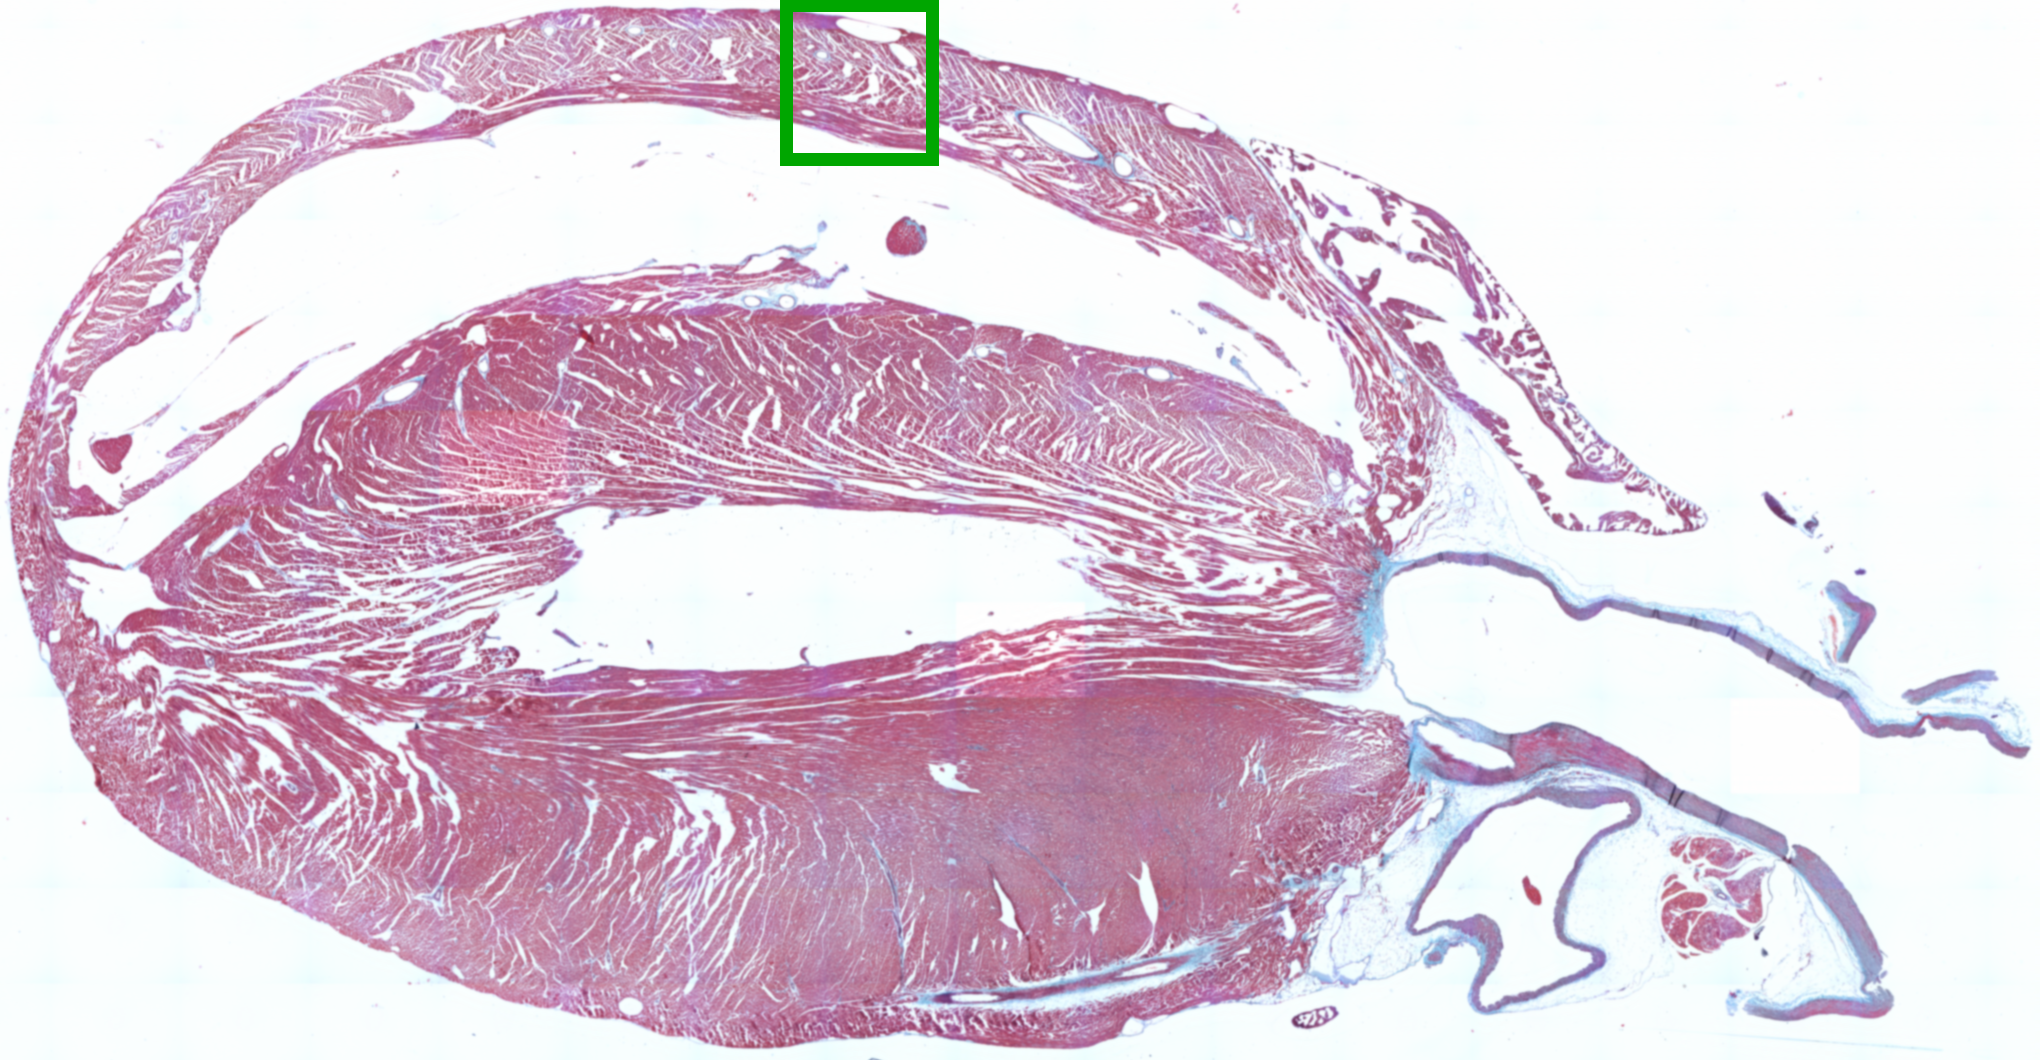
\includegraphics[width=1.7in]{2_methods/Figs/HiRes_downsamples_8_0582}}
      \subfloat[]{\includegraphics[width=1.7in]{2_methods/Figs/LoRes_rgb_downsamples_1_0582}}\\
      \subfloat[]{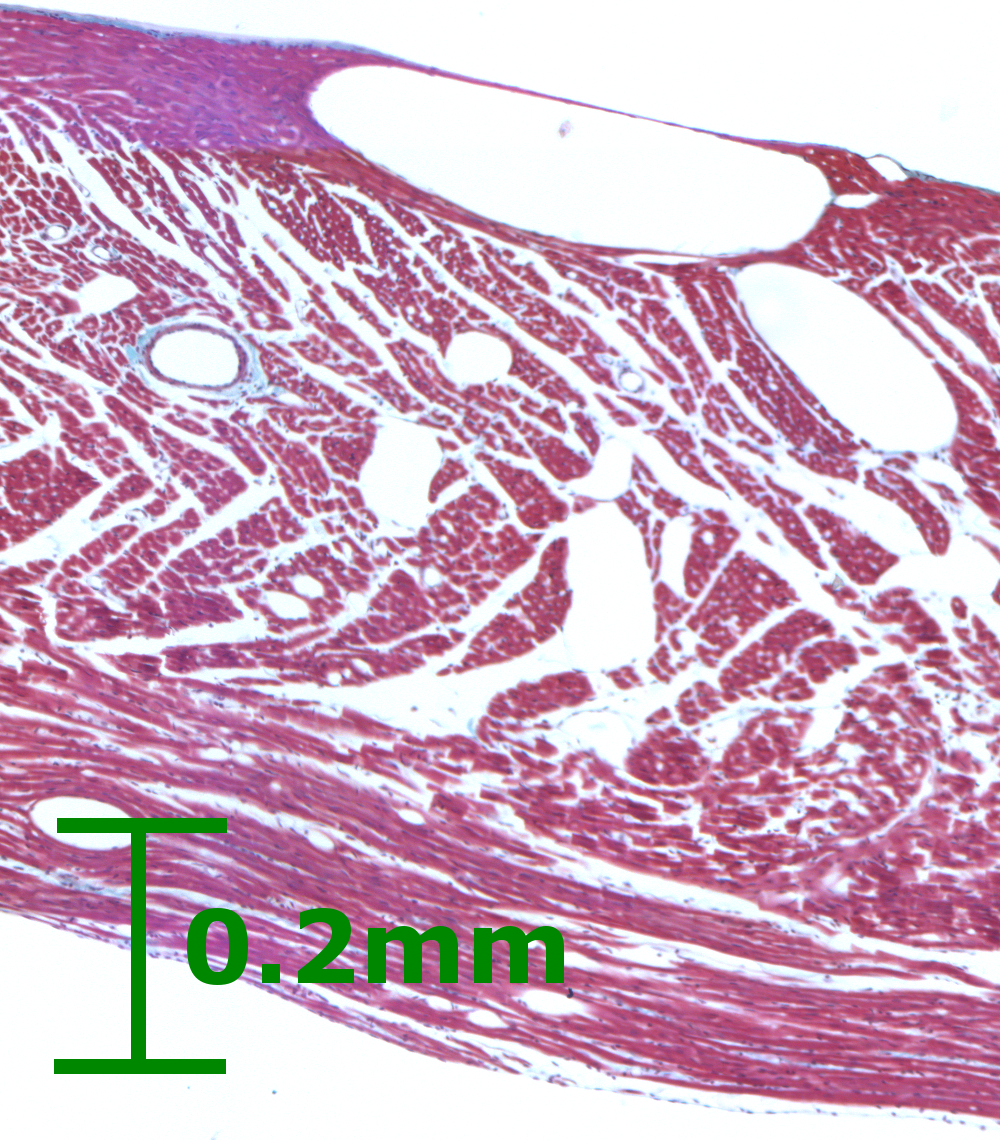
\includegraphics[width=1.7in]{2_methods/Figs/HiRes_downsamples_1_0582_zoom}}
      \subfloat[]{\includegraphics[width=1.7in]{2_methods/Figs/LoRes_rgb_downsamples_1_0582_zoom}}
      \caption{Figure on starting point, showing dataset images, whole and with zoom}
      \label{fig:raw_images}
    \end{figure}

    Hearts were isolated from female rats, fixed and embedded in black wax. The wax blocks were then serially sectioned at 10$\mu$m thickness using a microtome. An image of the top surface of the block -- referred to as a `block face image' from here on -- was taken with 25$\mu$m resolution after each slicing. Each slice was relaxed and rehydrated, before histology imaging was performed using a 5x objective with 1.1$\mu$m resolution, the resultant images being referred to as `histology images' from here on. Gibb et al. \cite{Gibb2012} give a more detailed account of the experimental methods. Examples of the block face and slice images are displayed in Figure~\ref{fig:raw_images}.
  % subsection image_acquisition (end)
  
  \subsection{Block Face Registration} % (fold)
  \label{sub:block_face_registration}
    All registration software developed for the work presented in this paper is based on ITK \cite{Yoo2002} and can be found at \cite{github_registration}. The ITK registration framework consists of the two images to be coregistered, and four main components: a transform, an interpolator, a fitness metric and an optimiser.
    
    Several sets of image downsamples of varying factors were generated, the lowest of which were used for debugging and testing, working up in detail, size and computational expense as the techniques were perfected. The histological images were initialised to their common geometrical centre to create an approximate volume, after which the volume was manually translated to align with the block face volume.
    
    A large proportion of the deformation introduced by the sectioning process is of similarity or affine form. By first registering the simplest of transforms with the lowest dimensional parameter space, and then incrementally relaxing transformational constraint by increasing the number of parameters, we can provide the best possible starting point in each higher dimensional parameter space. Transforms were therefore optimised in the following order, the final result of each initialising its successor: a centered rigid 2D transform - a rotation about an arbitrary centre followed by a translation; a centered similarity transform - as before but with a scaling factor; and a centered affine transform - an affine transformation around an arbitrary centre followed by a translation.

    A mean squares difference metric proved most robust over normalised correlation and mutual information. Parameter scalings were initially chosen based on the dimensions of the images, and subsequently tuned using diagnostic tools that output and visualised transforms and metric values at each iteration of the registration \cite{github_registration}. During registration of a small proportion of the slices, non-monotonicity in the gradient magnitude of the metric along the optimisation path caused the regular step gradient descent optimisation algorithm to reduce its scaling factor prematurely and fail to reach a global optimum. The gradient descent algorithm was therefore employed and yielded more consistent results. A linear interpolator was used to calculate off-grid pixel intensities in all cases.
  % subsection block_face_registration (end)
  
	\subsection{1-Dimensional Brownian Diffusion} % (fold)
	\label{sub:a_1d_random_walk_analogy}
    The central limit theorem states that the mean of a sufficiently large number of independent random variables will be approximately normally distributed, regardless of their individual distribution. Indeed, Einstein's theory of the Brownian motion of a diffusive particle is based on this precept. In particular, the de Moivre-Laplace Theorem states that in the large limit, and in the neighbourhood of the distribution peak, the binomial distribution approximates a Gaussian. In this light, we might consider a concentration of particles $f$ over a discrete 1-dimensional grid $x$, where after a small discretised timestep $\Delta t$, a proportion $2\alpha \Delta t$ of the particles take one step, such that half of them have diffused to the left and half to the right:
	  \begin{equation}
      \begin{split}
  	    f(x_i, t_{n+1}) = f(x_i, t_n) + \alpha (& f(x_{i-1}, t_n) \\
                                                & - 2f(x_i, t_n) \\
                                                & + f(x_{i+1}, t_n)).
      \end{split}
      \label{eqn:diffusion_1d}
		\end{equation}
	  This diffusion will of course act to smooth and homogenise $f$, since regions of high concentration relative to their neighbours will be reduced, and those of low concentration augmented. Since the particles move binomially, in accordance with the de Moivre Laplace Theorem it can be shown that multiple application of this smoothing operation approximates a Gaussian diffusion smoothing.
	% subsection a_1d_random_walk_analogy (end)
	
  \subsection{Transformational Diffusion Smoothing} % (fold)
  \label{sub:transformational_diffusion_smoothing}
    \subsubsection{Algorithm Overview} % (fold)
    \label{ssub:algorithm_overview}
    Our goal is to develop an iterative process that `diffuses' each histological slice image toward its neighbours, in order to smooth out high-frequency transformational noise, whilst maintaining the low-frequency underlying geometry of the volume. A transform $\mathbf{T}$ acting on a point $\mathbf{p}$ maps points in the resampling space to points in the original image space:
  		\begin{equation}
  			\mathbf{p'} = \mathbf{Tp}.
  		\end{equation}
    At iteration $n$ of the proposed process, each slice $i$ in a reconstructed histological stack has associated with it an invertible transform $\mathbf{T}_i^n$. We define the `diffusion transform' $\mathbf{\Delta T}_i^{n,n+1}$, which is formulated to move slice $i$ towards slices $i-1$ and $i+1$, based on the results of registrations between adjacent slices. $\mathbf{\Delta T}_i^{n,n+1}$ is pre-applied to a point in the resampling space of $i$ before $\mathbf{T}_i^n$ to give the adjusted transform $\mathbf{T}_i^{n+1}$, such that
    	\begin{equation}
  			\mathbf{T}_i^{n+1} = \mathbf{T}_i^n \mathbf{\Delta T}_i^{n,n+1}. \label{eqn:adjusted_transforms}
  		\end{equation}
	  It remains to formulate $\mathbf{\Delta T}_i^{n,n+1}$, and this is the subject of the following discussion.
    % subsubsection algorithm_overview (end)
    
    \subsubsection{Formulating the Diffusion Transforms} % (fold)
    \label{ssub:formulating_the_diffusion_transforms}
      In the case of 1-dimensional diffusion, we can reformulate the right hand side of (\ref{eqn:diffusion_1d}) into two separate terms thusly:
	  \begin{alignat}{2}
  	  f(x_i, t_{n+1}) &=\begin{aligned}
        % 1 &+ 2 \\
        % 3 &+ 4
        f(x_i, t_n) + \alpha (&(f(x_{i+1}, t_n) - f(x_i, t_n)) \\
                                    - &(f(x_{i-1}, t_n) - f(x_i, t_n))
  	  \end{aligned} \\
      \Delta f_i^{n,n+1} &= \alpha (\Delta f_{i,i+1}^n - \Delta f_{i-1,i}^n) \\
                         &= \alpha \Delta f_{i,i-1}^n + \alpha \Delta f_{i,i+1}^n, \label{eqn:1d_diffusion_operator}
		\end{alignat}
    where $\Delta f_i^{m,n}$ is the difference in $f$ at position $i$ between timestep $m$ and timestep $n$, and $\Delta f_{i,j}^m$ is the difference in $f$ between position $i$ and position $j$ at timestep $m$. From (\ref{eqn:1d_diffusion_operator}), we can see that at each timestep, the concentration at each bin moves towards its left and right neighbour by a proportion $\alpha$ of its difference from each, respectively.
		
	  We might, then, propose analogously that
		\begin{equation}
		 	\mathbf{\Delta T}_i^{n,n+1} = \alpha \cdot \mathbf{\Delta T}_{i,i+1}^n \oplus \alpha \cdot \mathbf{\Delta T}_{i,i-1}^n, \label{eqn:transformational_placeholder}
		\end{equation}
	 	where $\mathbf{\Delta T}_{i,j}^n = (\mathbf{\Delta T}_{j,i}^n)^{-1}$ is defined as the transformation that registers a histological slice $i$ to slice $j$ at iteration $n$, operator $\cdot$ is a placeholder for a binary operator on a scalar and a transform, and operator $\oplus$ is a placeholder for a binary operator on a pair of transforms. We are now equipped to calculate the transforms for progressively smoother and smoother volumes, by first registering each slice to its neighbour to obtain $\mathbf{\Delta T}_{i,i+1}^n$, then computing the diffusion transforms $\mathbf{\Delta T}_i^{n,n+1}$ through \labelcref{eqn:transformational_placeholder}, and finally applying them to the original transforms through \labelcref{eqn:adjusted_transforms} to obtain $\mathbf{T}_i^{n+1}$. The question now emerges: what precise form do the two binary operators take? We will start by outlining their desirable properties, and then discuss implementations that satisfy these constraints.
    % subsubsection formulating_the_diffusion_transforms (end)
		
    \subsubsection{Formulating the Transform Operators} % (fold)
    \label{ssub:formulating_the_transform_operators}
		The operator $\cdot$ takes two operands: a scalar and a transform. We would like $0$ to be the null operand on $\mathbf{T}$, so that when $\alpha = 0$, no diffusion occurs. We would like $1$ to be the identity operand on $\mathbf{T}$, so that when $\alpha = 1$, the transform from each term in (\ref{eqn:transformational_placeholder}) would diffuse the slice exactly to the position of its equivalent neighbour. Ideally, we would also like addition of the scalar operand to distribute over the serial application of the resultant transforms, so that transforms vary smoothly and naturally with respect to the scalar operand. This final condition can be satisfied for certain transforms, such as linear transforms and vector field transforms, but cannot be satisfied in general for others, such as b-spline transforms. To summarise in mathematical form, we would like the following to hold:
		\begin{gather}
			0 \cdot \mathbf{T} = \mathbf{I} \label{eqn:null} \\
			1 \cdot \mathbf{T} = \mathbf{T} \label{eqn:identity} \\
			(\alpha \cdot \mathbf{T}) (\beta \cdot \mathbf{T}) = (\alpha + \beta) \cdot \mathbf{T} \label{eqn:distributivity}
		\end{gather}
	 	
	  The operator $\oplus$ takes two transform operands. Commutativity must hold if the diffusion is to be symmetric i.e. behave identically if the order of the slices is reversed. If statistics are to be calculated on more than two transformations, it is also necessary for associativity to hold, so that the order of application of operator $\oplus$ is not preferential to any subset of transform operands. That is,
		\begin{gather}
			\forall \mathbf{S}, \mathbf{T} : \mathbf{S} \oplus \mathbf{T} = \mathbf{T} \oplus \mathbf{S} \label{eqn:commutativity} \\
			\forall \mathbf{S}, \mathbf{T} : (\mathbf{S} \oplus \mathbf{T}) \oplus \mathbf{U} = \mathbf{S} \oplus (\mathbf{T} \oplus \mathbf{U}). \label{eqn:associativity}
		\end{gather}
		Unfortunately, commutativity rules out the straightforward serial application of transforms. For example, in the general case of matrix multiplication, $AB \ne BA$. One solution is to use the transform that is equivalent to returning the Euclidian midpoint of $\mathbf{Sp}$ and $\mathbf{Tp}$ for all $\mathbf{p}$. However, the result may not always be representable by some types of transform (notably b-spline transforms), and further, it may be dependent on the order that the $\oplus$ operator is applied. In group theoretical terms, two axioms of the group $(\mathbf{T},\oplus)$ are violated: closure and associativity. Aside from anything else, the Euclidian midpoint approach leads in many cases to unnatural results, such as the `bulging' effect noted in \cite{Arsigny2005a}, and the null matrix in 2D between transforms separated by a rotation of $\pi$.
        
	  It is elucidating to consider the general mathematical form constrained by \labelcref{eqn:null,eqn:identity,eqn:distributivity,eqn:commutativity,eqn:distributivity} applied to concrete classes of transform, in order of increasing complexity: translation transforms, rotation transforms, similarity transforms, affine transforms and more general deformable transforms. An affine transform $\mathbf{T}$ acting on a point $\mathbf{p}$ consists of a matrix transformation $\mathbf{M}$, followed by a translation by an offset vector $\mathbf{o}$:
		\begin{equation}
			\mathbf{p'} = \mathbf{Tp}= \mathbf{Mp} + \mathbf{o}.
		\end{equation}
		In the simplest case of translation transforms, where $\mathbf{M}$ is the identity matrix $\mathbf{I}$ i.e. $\mathbf{Tp} = \mathbf{p} + \mathbf{o}$, the two translation parameters are independent and individually identical to the 1-dimensional diffusion in (\ref{eqn:1d_diffusion_operator}). Operator $\cdot$ is a scalar multiplication of each offset parameter, and operator $\oplus$ is the commutative serial application of the transforms (or equivalently, addition of the respective parameters):
		\begin{align}
			(\alpha \cdot \mathbf{T}) \mathbf{p} &= \mathbf{p} + \alpha\mathbf{o} \label{eqn:translation_cdot}\\
			(\mathbf{S} \oplus \mathbf{T}) \mathbf{p} &= \mathbf{STp} \\
			                                          &= \mathbf{p} + \mathbf{o_S} + \mathbf{o_T} \label{eqn:translation_oplus}
		\end{align}
		Clearly, these two operators satisfy \labelcref{eqn:null,eqn:identity,eqn:distributivity,eqn:commutativity,eqn:associativity}. (\ref{eqn:transformational_placeholder}) becomes
		\begin{align}
		 	\mathbf{\Delta T}_i^{n,n+1} \mathbf{p} &= (\alpha \mathbf{\Delta T}_{i,i-1}^n) (\alpha \mathbf{\Delta T}_{i,i+1}^n) \mathbf{p} \\
			\mathbf{p} + \mathbf{o}_i^{n,n+1} &= \mathbf{p} + \alpha \mathbf{o}_{i,i-1}^n + \alpha \mathbf{o}_{i,i+1}^n \\
			\mathbf{o}_i^{n,n+1} &= \alpha (\mathbf{o}_{i,i-1}^n + \mathbf{o}_{i,i+1}^n) 
		\end{align}
		The offsets are therefore trivially analogous to (\ref{eqn:1d_diffusion_operator}).
		
		In the case of rigid transforms, $\mathbf{M}$ is a rotation matrix $\mathbf{R}(\theta)$. In 2 dimensions, rotation matrices commute, and the result of their multiplication is simply a rotation matrix with angle equal to the sum of the operands' angles; in the special case where there are no offsets, then serial application of the transforms is a candidate for operator $\oplus$ according to (\ref{eqn:commutativity}):
		\begin{equation}
			\mathbf{S} \oplus \mathbf{T} = \mathbf{R}(\theta_\mathbf{S})\mathbf{R}(\theta_\mathbf{T}) = \mathbf{R}(\theta_\mathbf{S} + \theta_\mathbf{T}) = \mathbf{T} \oplus \mathbf{S}
		\end{equation}
		In a similar vein, an operator $\cdot$ that multiplies the angle of the input transform with $\alpha$ fulfils criteria \labelcref{eqn:null,eqn:identity,eqn:distributivity}:
    \begin{equation}
      \alpha \cdot \mathbf{T} = \mathbf{R}(\alpha\theta).
    \end{equation}
		
        In the case of similarity transforms with no offset, $\mathbf{M}$ is a rotation matrix $\mathbf{R}$ multiplied by an enlargement $\sigma$:
        \begin{equation}
            \mathbf{T} = \sigma\mathbf{R}(\theta).
        \end{equation}
        Since scalar multiplications commute with matrix transformations, if the operator $\cdot$ is constructed to scale geometrically, the situation is very similar to that of rotation matrices and \labelcref{eqn:null,eqn:identity,eqn:distributivity,eqn:commutativity,eqn:associativity} still apply:
        \begin{gather}
          \alpha \cdot \mathbf{T} = \sigma^{\alpha}\mathbf{R}(\alpha\theta) \\
          \begin{split}
            (\alpha \cdot \mathbf{T})(\beta \cdot \mathbf{T}) &= \sigma^{\alpha + \beta}\mathbf{R}((\alpha + \beta)\theta) \\
                                                              &= (\alpha + \beta) \cdot \mathbf{T}
          \end{split} \\
          \mathbf{S} \oplus \mathbf{T} = \sigma_\mathbf{S}\mathbf{R}(\theta_\mathbf{S})\sigma_\mathbf{T}\mathbf{R}(\theta_\mathbf{T}) = \mathbf{T} \oplus \mathbf{S} \\
          \begin{split}
      			(\mathbf{S} \oplus \mathbf{T}) \oplus \mathbf{U} &= \sigma_\mathbf{S}\sigma_\mathbf{T}\sigma_\mathbf{U}\mathbf{R}(\theta_\mathbf{S} + \theta_\mathbf{T} + \theta_\mathbf{U}) \\
                                                             &= \mathbf{S} \oplus (\mathbf{T} \oplus \mathbf{U}).
          \end{split}
        \end{gather}
		
		In the more general case of diagonalisable affine matrix transformations, in the absence of translations, and when $\mathbf{S}$ and $\mathbf{T}$ can be diagonalised by the same matrix $\mathbf{V}$ i.e. $\mathbf{S} = \mathbf{VD_SV}^{-1}$ and $\mathbf{T} = \mathbf{VD_TV}^{-1}$, commutativity still holds for serial application:
        \begin{equation}
          \begin{split}
      			\mathbf{S} \oplus \mathbf{T} &= \mathbf{ST} \\
                                         &= \mathbf{VD_SV}^{-1}\mathbf{VD_TV}^{-1} \\
                                         &= \mathbf{VD_SD_TV}^{-1} \\
                                         &= \mathbf{VD_TD_SV}^{-1} \\
                                         &= \mathbf{T} \oplus \mathbf{S},
          \end{split}
        \end{equation}
        with associativity of course holding for the serial application of affine transformations in general. However, when $\mathbf{M_S}$ and $\mathbf{M_T}$ no longer commute, serial application of transforms is no longer sufficient. There is also no obvious form of operator $\cdot$ which satisfies \labelcref{eqn:null,eqn:identity,eqn:distributivity}. We must take recourse to a more general formulation of operators $\cdot$ and $\oplus$.
        
        It is here that we must introduce the concept of the matrix exponential:
        \begin{equation}
          e^{\mathbf{M}} = \sum_{k=0}^{\infty}\frac{1}{k!}\mathbf{M}^k. \label{eqn:matrix_exponential}
        \end{equation}
        Conversely, a logarithm $\mathbf{L}$ of a matrix $\mathbf{M}$ is another matrix such that $e^\mathbf{L} = \mathbf{M}$. For any invertible matrix $\mathbf{Y}$, it is clear that
        \begin{gather}
          (\mathbf{YM}\mathbf{Y}^{-1})^n = \mathbf{Y}\mathbf{M}^n\mathbf{Y}^{-1}, n \in \mathbb{N}.
        \end{gather}
        It then follows from (\ref{eqn:matrix_exponential}) that
        \begin{align}
          \mathbf{Y}e^{\mathbf{M}}\mathbf{Y}^{-1} &= \mathbf{Y}\left(\sum_{k=0}^{\infty}\frac{1}{k!}\mathbf{M}^k\right)\mathbf{Y}^{-1} \\
                                                  &= \sum_{k=0}^{\infty}\frac{1}{k!}\mathbf{Y}\mathbf{M}^k\mathbf{Y}^{-1} \\
                                                  &= \sum_{k=0}^{\infty}\frac{1}{k!}(\mathbf{YM}\mathbf{Y}^{-1})^k \label{eqn:diagonal_exp} \\
                                                  &= e^{\mathbf{YM}\mathbf{Y}^{-1}}.
        \end{align}
        If $\mathbf{M}$ is diagonalisable, and we choose a $\mathbf{Y}$ that diagonalises $\mathbf{M}$, such that $\mathbf{D} = \mathbf{YMY}^{-1}$, (\ref{eqn:diagonal_exp}) becomes trivially analogous to the Taylor expansion for a scalar exponential, and we can then simply compute the exponential of each diagonal element of $\mathbf{D}$. It follows that the logarithm of a positive definite diagonal matrix can be computed by taking the logarithm of each of its elements.
        
        It turns out that when a matrix $\mathbf{M}$ has a logarithm $\mathbf{L}$, $\mathbf{M}$ is in a Lie group --- a group on a smooth manifold. $\mathbf{L}$ is the corresponding element of the associated Lie algebra. $\mathbf{L}$ is an `infinitessimal generator', and its value determines the tangent space at the identity $\mathbf{I}$. Informally, this means that there exists a matrix $\mathbf{I} + \epsilon \mathbf{L}$ that is extremely close to the identity, such that when applied repeatedly an extremely large number of times i.e. $(\mathbf{I} + \epsilon \mathbf{L})^n$, the result eventually becomes $\mathbf{M}$.
        
        If we define operator $\cdot$ in terms of the exponential and the logarithm of $\mathbf{M}$, \labelcref{eqn:null,eqn:identity,eqn:distributivity} are all satisfied:
        \begin{gather}
          \alpha \cdot \mathbf{M} = e^{\alpha\ln\mathbf{M}} \\
          0 \cdot \mathbf{M} = e^0 = \mathbf{I} \\
          1 \cdot \mathbf{M} = e^{\ln\mathbf{M}} = \mathbf{M} \\
          \begin{split}
            (\alpha \cdot \mathbf{M})(\beta \cdot \mathbf{M}) &= e^{\alpha\ln\mathbf{M}}e^{\beta\ln\mathbf{M}} \\
                                                              &= e^{(\alpha + \beta)\ln\mathbf{M}} \\
                                                              &= (\alpha + \beta) \cdot \mathbf{M}.
          \end{split}
        \end{gather}
        We can define operator $\oplus$ as a simple addition of the matrix logarithms in log-Euclidian space, followed by a mapping back to transform space with the exponential operator:
        \begin{equation}
          \mathbf{M_S} \oplus \mathbf{M_T} = e^{\ln\mathbf{M_S} + \ln\mathbf{M_T}}.
        \end{equation}
        Because all operations are homomorphic with Euclidian vector space, this operator always fulfils the commutativity and associativity criteria
        \begin{gather}
          \mathbf{M_S} \oplus \mathbf{M_T} = e^{\ln\mathbf{M_S} + \ln\mathbf{M_T}} = \mathbf{M_T} \oplus \mathbf{M_S} \\
          \begin{split}
            (\mathbf{M_S}\oplus\mathbf{M_T})\oplus\mathbf{M_U} &= e^{\ln\mathbf{M_S} + \ln\mathbf{M_T} + \ln\mathbf{M_U}} \\
                                                               &= \mathbf{M_S}\oplus(\mathbf{M_T}\oplus\mathbf{M_U}).
          \end{split}
        \end{gather}
        It is pleasing to note that this new formula coincides with the special cases of rotation, similarity and diagonalisability discussed previously, since whenever the two matrices commute,
        \begin{equation}
          \begin{split}
            \mathbf{M_SM_T} &= e^{\ln\mathbf{M_S}}e^{\ln\mathbf{M_T}} \\
                            &= e^{\ln\mathbf{M_S} + \ln\mathbf{M_T}} \\
                            &= \mathbf{M_S} \oplus \mathbf{M_T}.
          \end{split}
        \end{equation}
        This `log-Euclidian' approach is expounded with Titanic mathematical rigour in \cite{Arsigny2005}. However, being motivated by the interpolation of MRI data, the treatise is limited to tensors; that is, symmetric matrices with no translation.
        
		    So far, the discussion has been limited to cases with zero offset. When offsets are introduced, even when their respective matrices commute, the commutativity of transforms in (\ref{eqn:commutativity}) no longer holds when serial action akin to (\ref{eqn:translation_oplus}) is introduced na\"ively:
        \begin{equation}
          (\mathbf{S} \oplus \mathbf{T})\mathbf{p} = (\mathbf{M_S} \oplus \mathbf{M_T})\mathbf{p} + \mathbf{M_So_T} + \mathbf{o_S} \ne (\mathbf{T} \oplus \mathbf{S})\mathbf{p}.
        \end{equation}
        If commutivity is forced, by averaging the offset contributions from both permutations of the operands i.e.
        \begin{equation}
          \begin{split}
            (\mathbf{S} \oplus \mathbf{T})\mathbf{p} &= (\mathbf{T} \oplus \mathbf{S})\mathbf{p} \\
                                                     &= (\mathbf{M_S} \oplus \mathbf{M_T})\mathbf{p} \\
                                                     &\qquad + \frac{1}{2}\left(\left( \mathbf{M_S} + \mathbf{I} \right) \mathbf{o_T} + \left( \mathbf{M_T} + \mathbf{I} \right)\mathbf{o_S}\right),
          \end{split}
        \end{equation}
        then associativity breaks down. The same underlying structure precludes a linear interpolation in operator $\cdot$ akin to \labelcref{eqn:translation_cdot} in the presence of a non-identical matrix:
        \begin{gather}
          (\alpha \cdot \mathbf{T})(\beta \cdot \mathbf{T})\mathbf{p} = \mathbf{M}_{\alpha+\beta}\mathbf{p} + \beta\mathbf{M}_{\alpha}\mathbf{o} + \alpha\mathbf{o} \ne (\alpha + \beta) \cdot \mathbf{T}.
        \end{gather}
        When $\mathbf{I} - \mathbf{M}$ is invertible --- that is, when none of the eigenvalues of $\mathbf{M}$ are equal to 1 --- we can express a transform as a matrix transformation about a single invariant centre, with no offset:
        \begin{gather}
          \mathbf{Tp} = \mathbf{Mp} + \mathbf{o} = \mathbf{M}(\mathbf{p}-\mathbf{c}) + \mathbf{c} \\
          \mathbf{o} = (\mathbf{I} - \mathbf{M})\mathbf{c} \\
          \mathbf{c} = (\mathbf{I} - \mathbf{M})^{-1}\mathbf{o}.
        \end{gather}
        We can then reformulate operator $\cdot$ as a log-Euclidian transformation about this invariant centre and satisfy distributivity:
        \begin{gather}
          \alpha \cdot \mathbf{T} = e^{\alpha\ln\mathbf{M}}(p - c) + c \label{eqn:affine_cdot} \\
          \begin{split}
            (\alpha \cdot \mathbf{T})(\beta \cdot \mathbf{T}) &= e^{\alpha\ln\mathbf{M}}((e^{\beta\ln\mathbf{M}}(p - c) + c) - c) + c \\
                                                              &= e^{\alpha\ln\mathbf{M}}(e^{\beta\ln\mathbf{M}}(p - c)) + c \\
                                                              &= e^{(\alpha + \beta)\ln\mathbf{M}}(p - c) + c \\
                                                              &= (\alpha + \beta) \cdot \mathbf{T}.
          \end{split}
        \end{gather}
        With this condition satisfied, $\alpha\cdot\mathbf{T}$ is equivalent to $\mathbf{T}^{\alpha}$.
        
        In order to derive the common centre of the two operands of operator $\oplus$, let us consider the infinitesimal case
        \begin{gather}
          \delta \cdot \mathbf{U} = (\delta \cdot \mathbf{S}) \oplus (\delta \cdot \mathbf{T}) \approx (\delta \cdot \mathbf{S}) (\delta \cdot \mathbf{T}) \\
          \begin{aligned}
            &e^{\delta(\ln \mathbf{M_S} + \ln \mathbf{M_T})}\mathbf{p} \\
            &+ (\mathbf{I} - e^{\delta(\ln \mathbf{M_S} + \ln \mathbf{M_T})})\mathbf{c_U}
          \end{aligned} = \begin{aligned}
              &e^{\delta \ln \mathbf{M_S}}e^{\delta \ln \mathbf{M_T}}\mathbf{p} \\
              &+ e^{\delta \ln \mathbf{M_S}}(\mathbf{I} - e^{\delta \ln \mathbf{T}})\mathbf{c_T} \\
              &+ (\mathbf{I} - e^{\delta \ln \mathbf{M_S}})\mathbf{c_S}. \label{eqn:infinitesimal_oplus}
          \end{aligned}
        \end{gather}
        We can see from the series in (\ref{eqn:matrix_exponential}) that
        \begin{equation}
          e^{\delta \ln \mathbf{M}} = \mathbf{I} + \delta \ln \mathbf{M} + \mathcal{O}((\delta \ln \mathbf{M})^2).
        \end{equation}
        Applying this to (\ref{eqn:infinitesimal_oplus}), we obtain
        \begin{equation}
          (\ln\mathbf{M_S} + \ln\mathbf{M_T})\mathbf{c_U} = (\ln\mathbf{M_S})\mathbf{c_S} + (\ln\mathbf{M_T})\mathbf{c_T}.
        \end{equation}
        The general form of operator $\oplus$ is then finally
        \begin{gather}
          \mathbf{S} \oplus \mathbf{T} = e^{\ln\mathbf{M_S} + \ln\mathbf{M_T}}(\mathbf{p} - \mathbf{c}) + \mathbf{c}, \nonumber \\
          \mathbf{c} = (\ln\mathbf{M_S} + \ln\mathbf{M_T})^{-1}((\ln\mathbf{M_S})\mathbf{c_S} + (\ln\mathbf{M_T})\mathbf{c_T}). \label{eqn:affine_oplus}
        \end{gather}
        Commutativity is evident by inspection, and associativity is simply demonstrated:
        \begin{gather}
          \begin{split}
            (\mathbf{S} \oplus \mathbf{T}) \oplus \mathbf{U} &= \exp(\ln(e^{\ln\mathbf{M_S} + \ln\mathbf{M_T}}) + \ln\mathbf{M_U})(\mathbf{p} - \mathbf{c}) \\
                                                             &\quad + \mathbf{c} \\
                                                             &= e^{\ln\mathbf{M_S} + \ln\mathbf{M_T} + \ln\mathbf{M_U}}(\mathbf{p} - \mathbf{c}) + \mathbf{c},
          \end{split} \\
          \begin{split}
            \mathbf{c} =& (\ln\mathbf{M_{S \oplus T}} + \ln\mathbf{M_U})^{-1} \\
                       &\quad ((\ln\mathbf{M_{S \oplus T}})\mathbf{c_{S \oplus T}} + (\ln\mathbf{M_U})\mathbf{c_U}) \\
                       =& (\ln\mathbf{M_S} + \ln\mathbf{M_T} + \ln\mathbf{M_U})^{-1} \\
                       &\quad ((\ln\mathbf{M_S})\mathbf{c_S} + (\ln\mathbf{M_T})\mathbf{c_T} + (\ln\mathbf{M_U})\mathbf{c_U}).
          \end{split}
        \end{gather}
        As a last algebraic-structural perk, it can be shown from \labelcref{eqn:affine_cdot,eqn:affine_oplus} that the operation of $\cdot$ by a scalar distributes over the operation of $\oplus$ on two affine transformations. In particular,
        \begin{equation}
          (\alpha \cdot \mathbf{S}) \oplus (\alpha \cdot \mathbf{T}) = \alpha \cdot (\mathbf{S} \oplus \mathbf{T}).
        \end{equation}
        
        In the case where $\mathbf{M} - \mathbf{I}$ is singular and there is no central invariate coordinate along the singular dimensions, it is of course natural that operator $\cdot$ interpolates the translation coordinates linearly along those dimensions as in (\ref{eqn:translation_cdot}), and that operator $\oplus$ sums translations arithmetically as in (\ref{eqn:translation_oplus}).
        
        A similar Lie theoretical approach must be taken when implementing operators $\cdot$ and $\oplus$ for more general non-rigid transforms, such as displacement field transforms. However, any differentiable transform will approximate an affine transformation at scales smaller than its curvature, and the implementations expounded here will suffice to smooth out those smaller subregions.
    % subsubsection formulating_the_transform_operators (end)
  % subsection transformational_diffusion_smoothing (end)
	
  \subsection{Diffusion on Synthetic Geometries} % (fold)
    \label{sub:diffusion_on_synthetic_geometries}
    In order to test the efficacy of the algorithm in a quantitative way, it was necessary to devise several test geometries. A stack of 200 identical histology slices is presented here, incorporating two low-frequency sinusoidal signals: a translational signal of amplitude approximately half the dimension of the heart section, and a rotational signal spanning 90$^{\circ}$, out of phase with the translational signal by by 90$^{\circ}$. The transform parameters of each slice are then purturbed by random Gaussian noise, with translational $\sigma$ equal to half the amplitude of the translational signal, and the affine matrix element $\sigma$ equal to 0.1.
  
  \begin{figure}[!t]
    \centering
    \subfloat[]{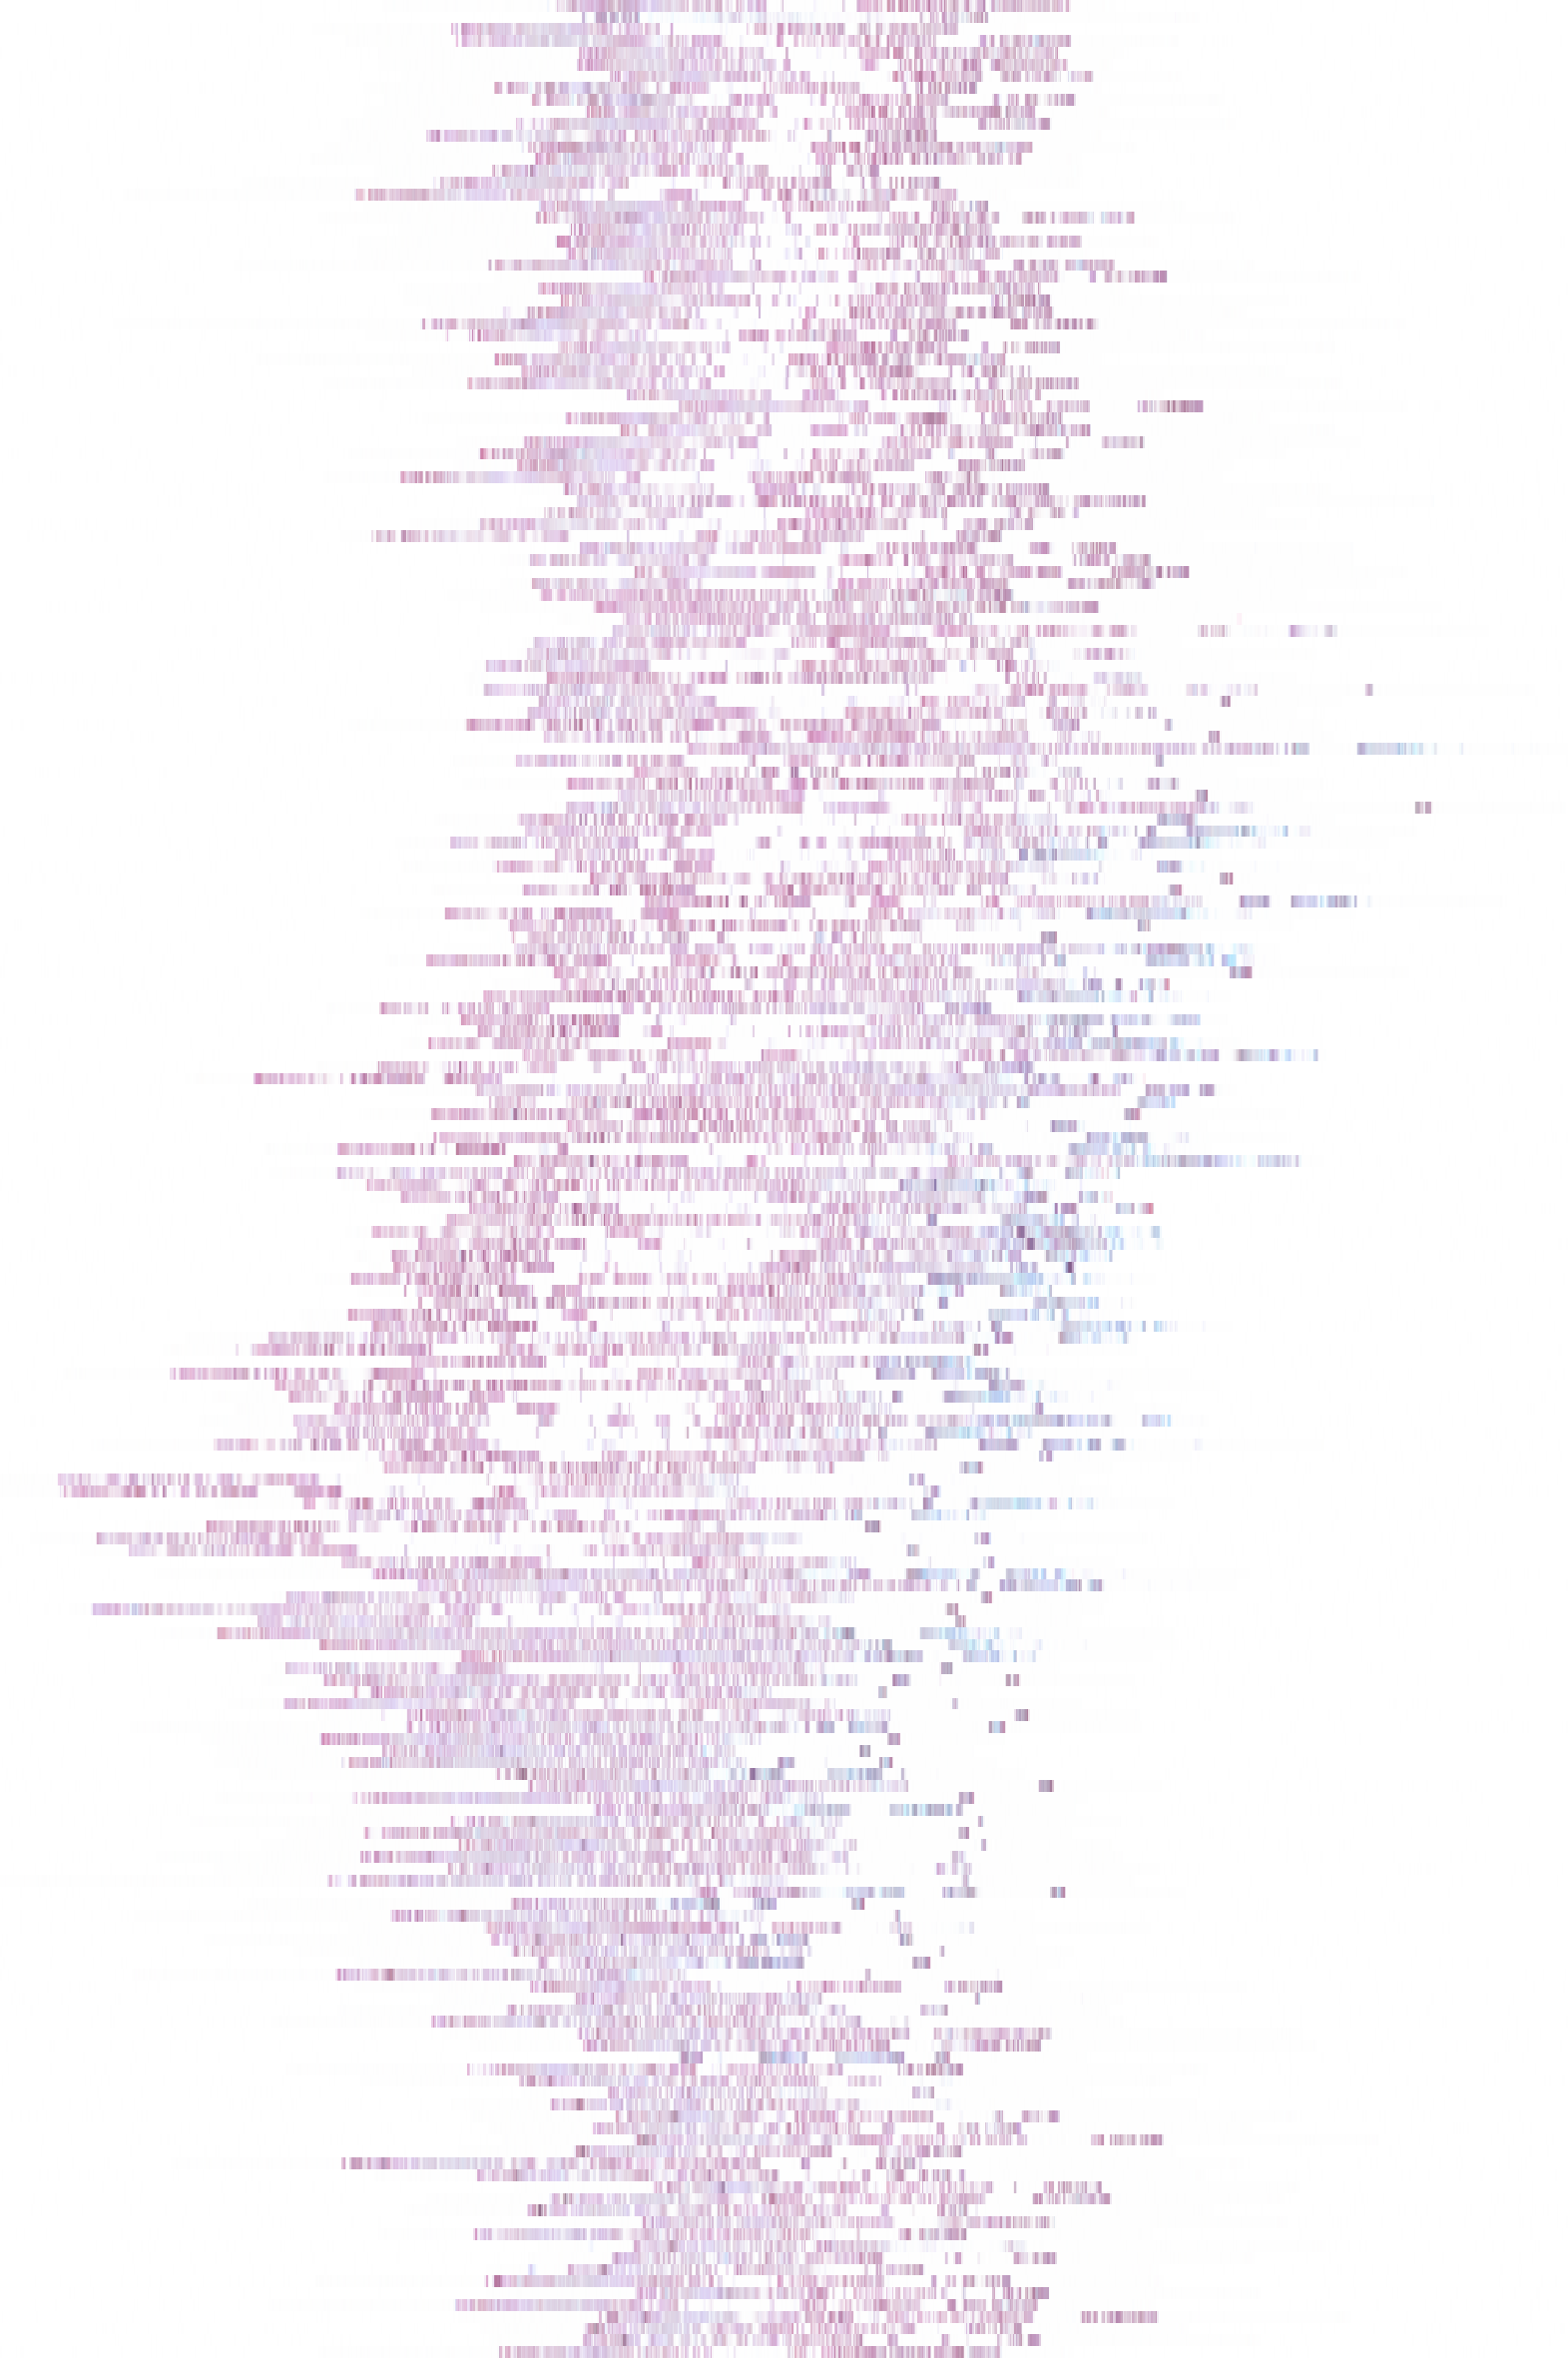
\includegraphics[width=1.1in]{2_methods/Figs/cross_section_0}\label{fig:synthetic_cross_section_0}}
    \subfloat[]{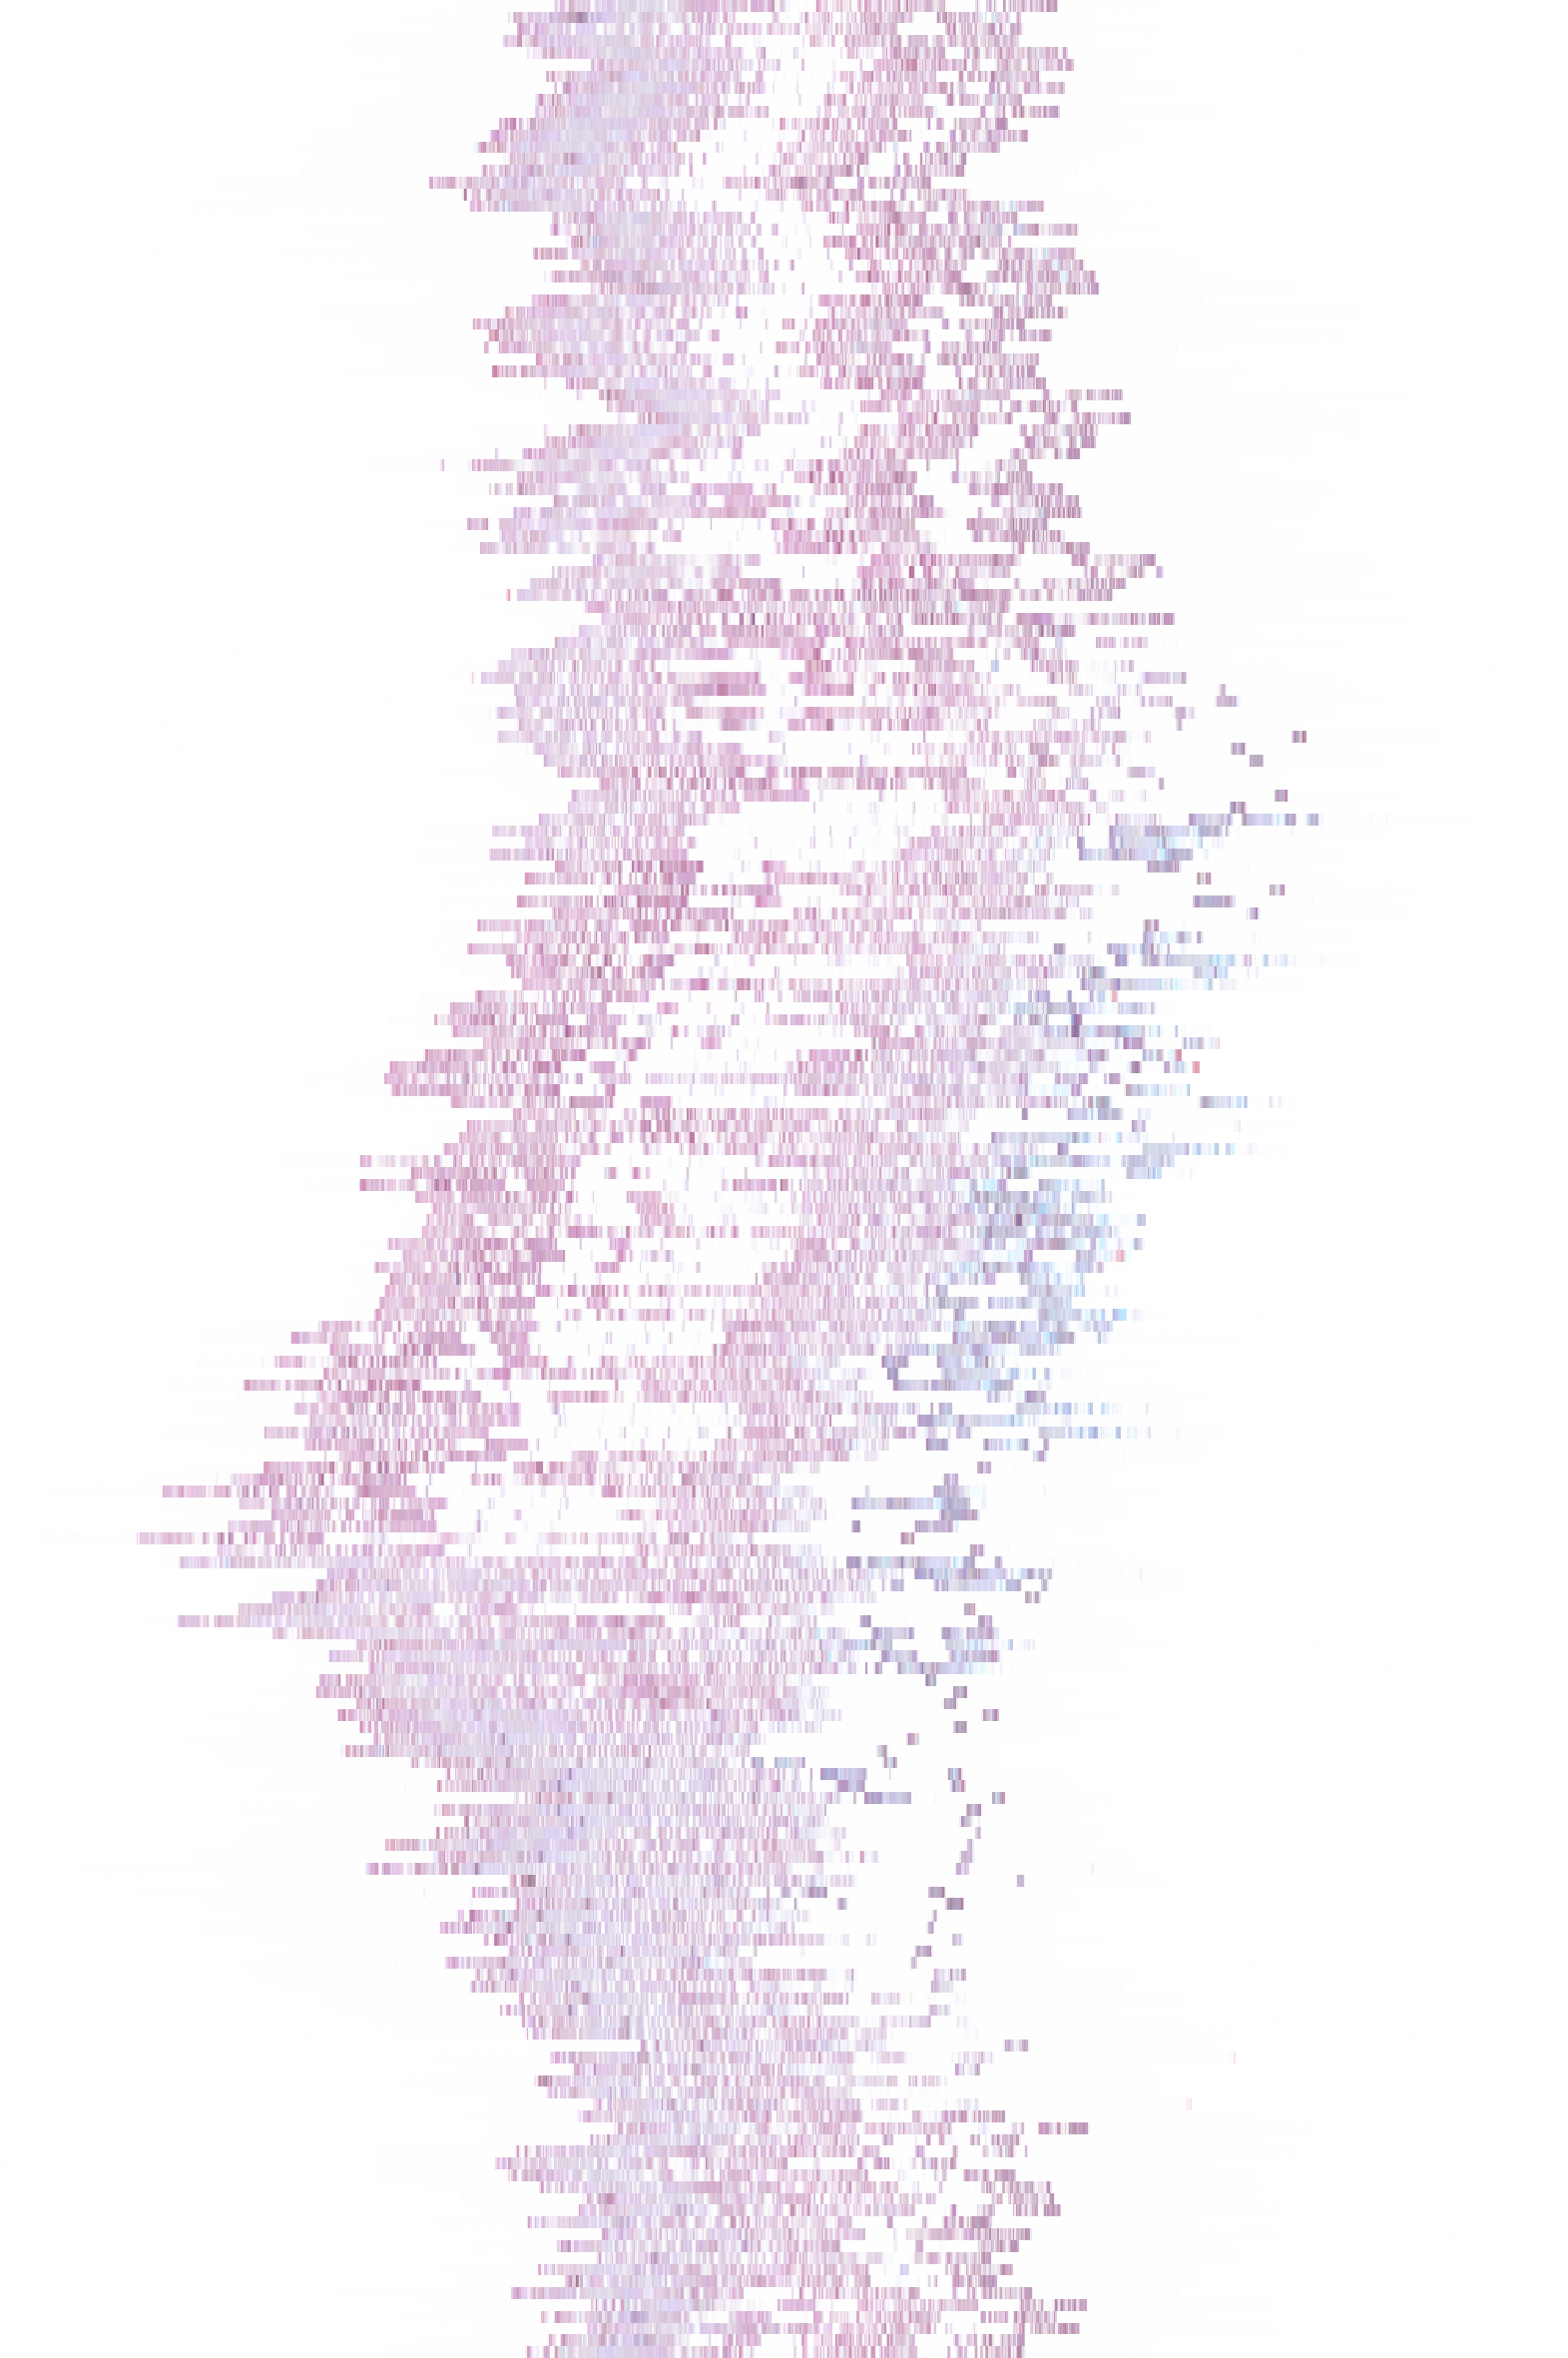
\includegraphics[width=1.1in]{2_methods/Figs/cross_section_1}}
    \subfloat[]{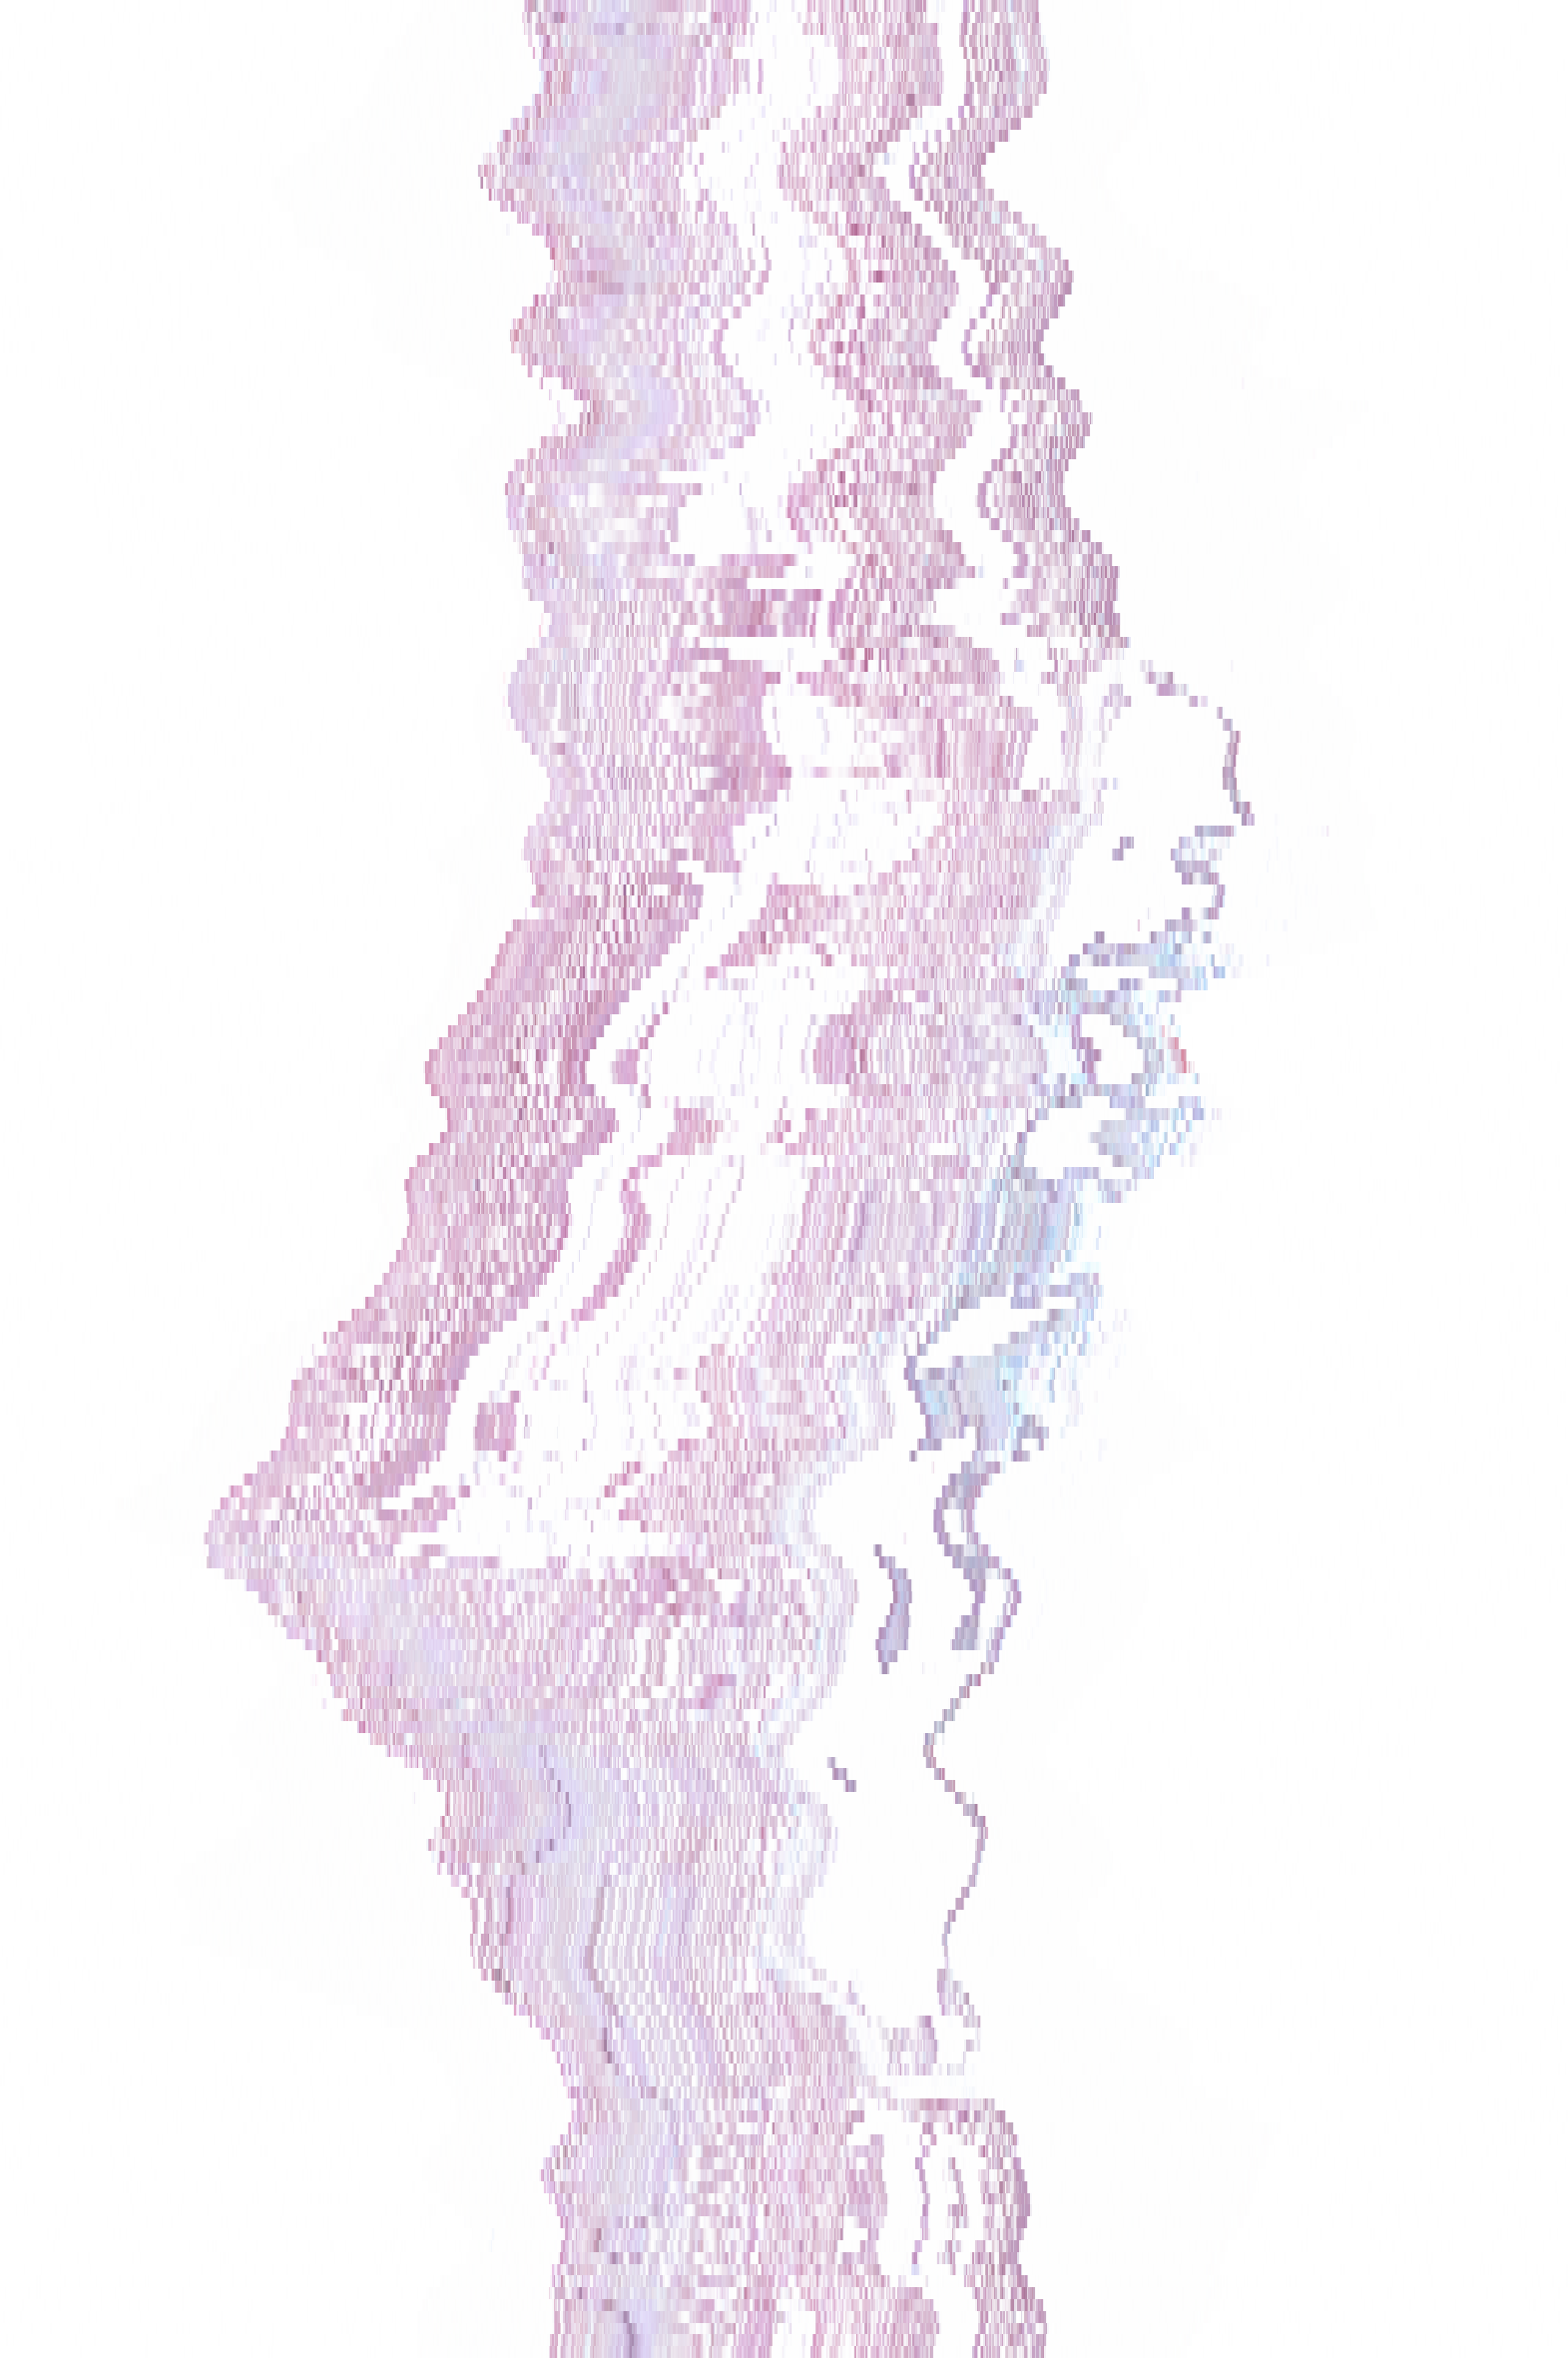
\includegraphics[width=1.1in]{2_methods/Figs/cross_section_7}}\\
    \subfloat[]{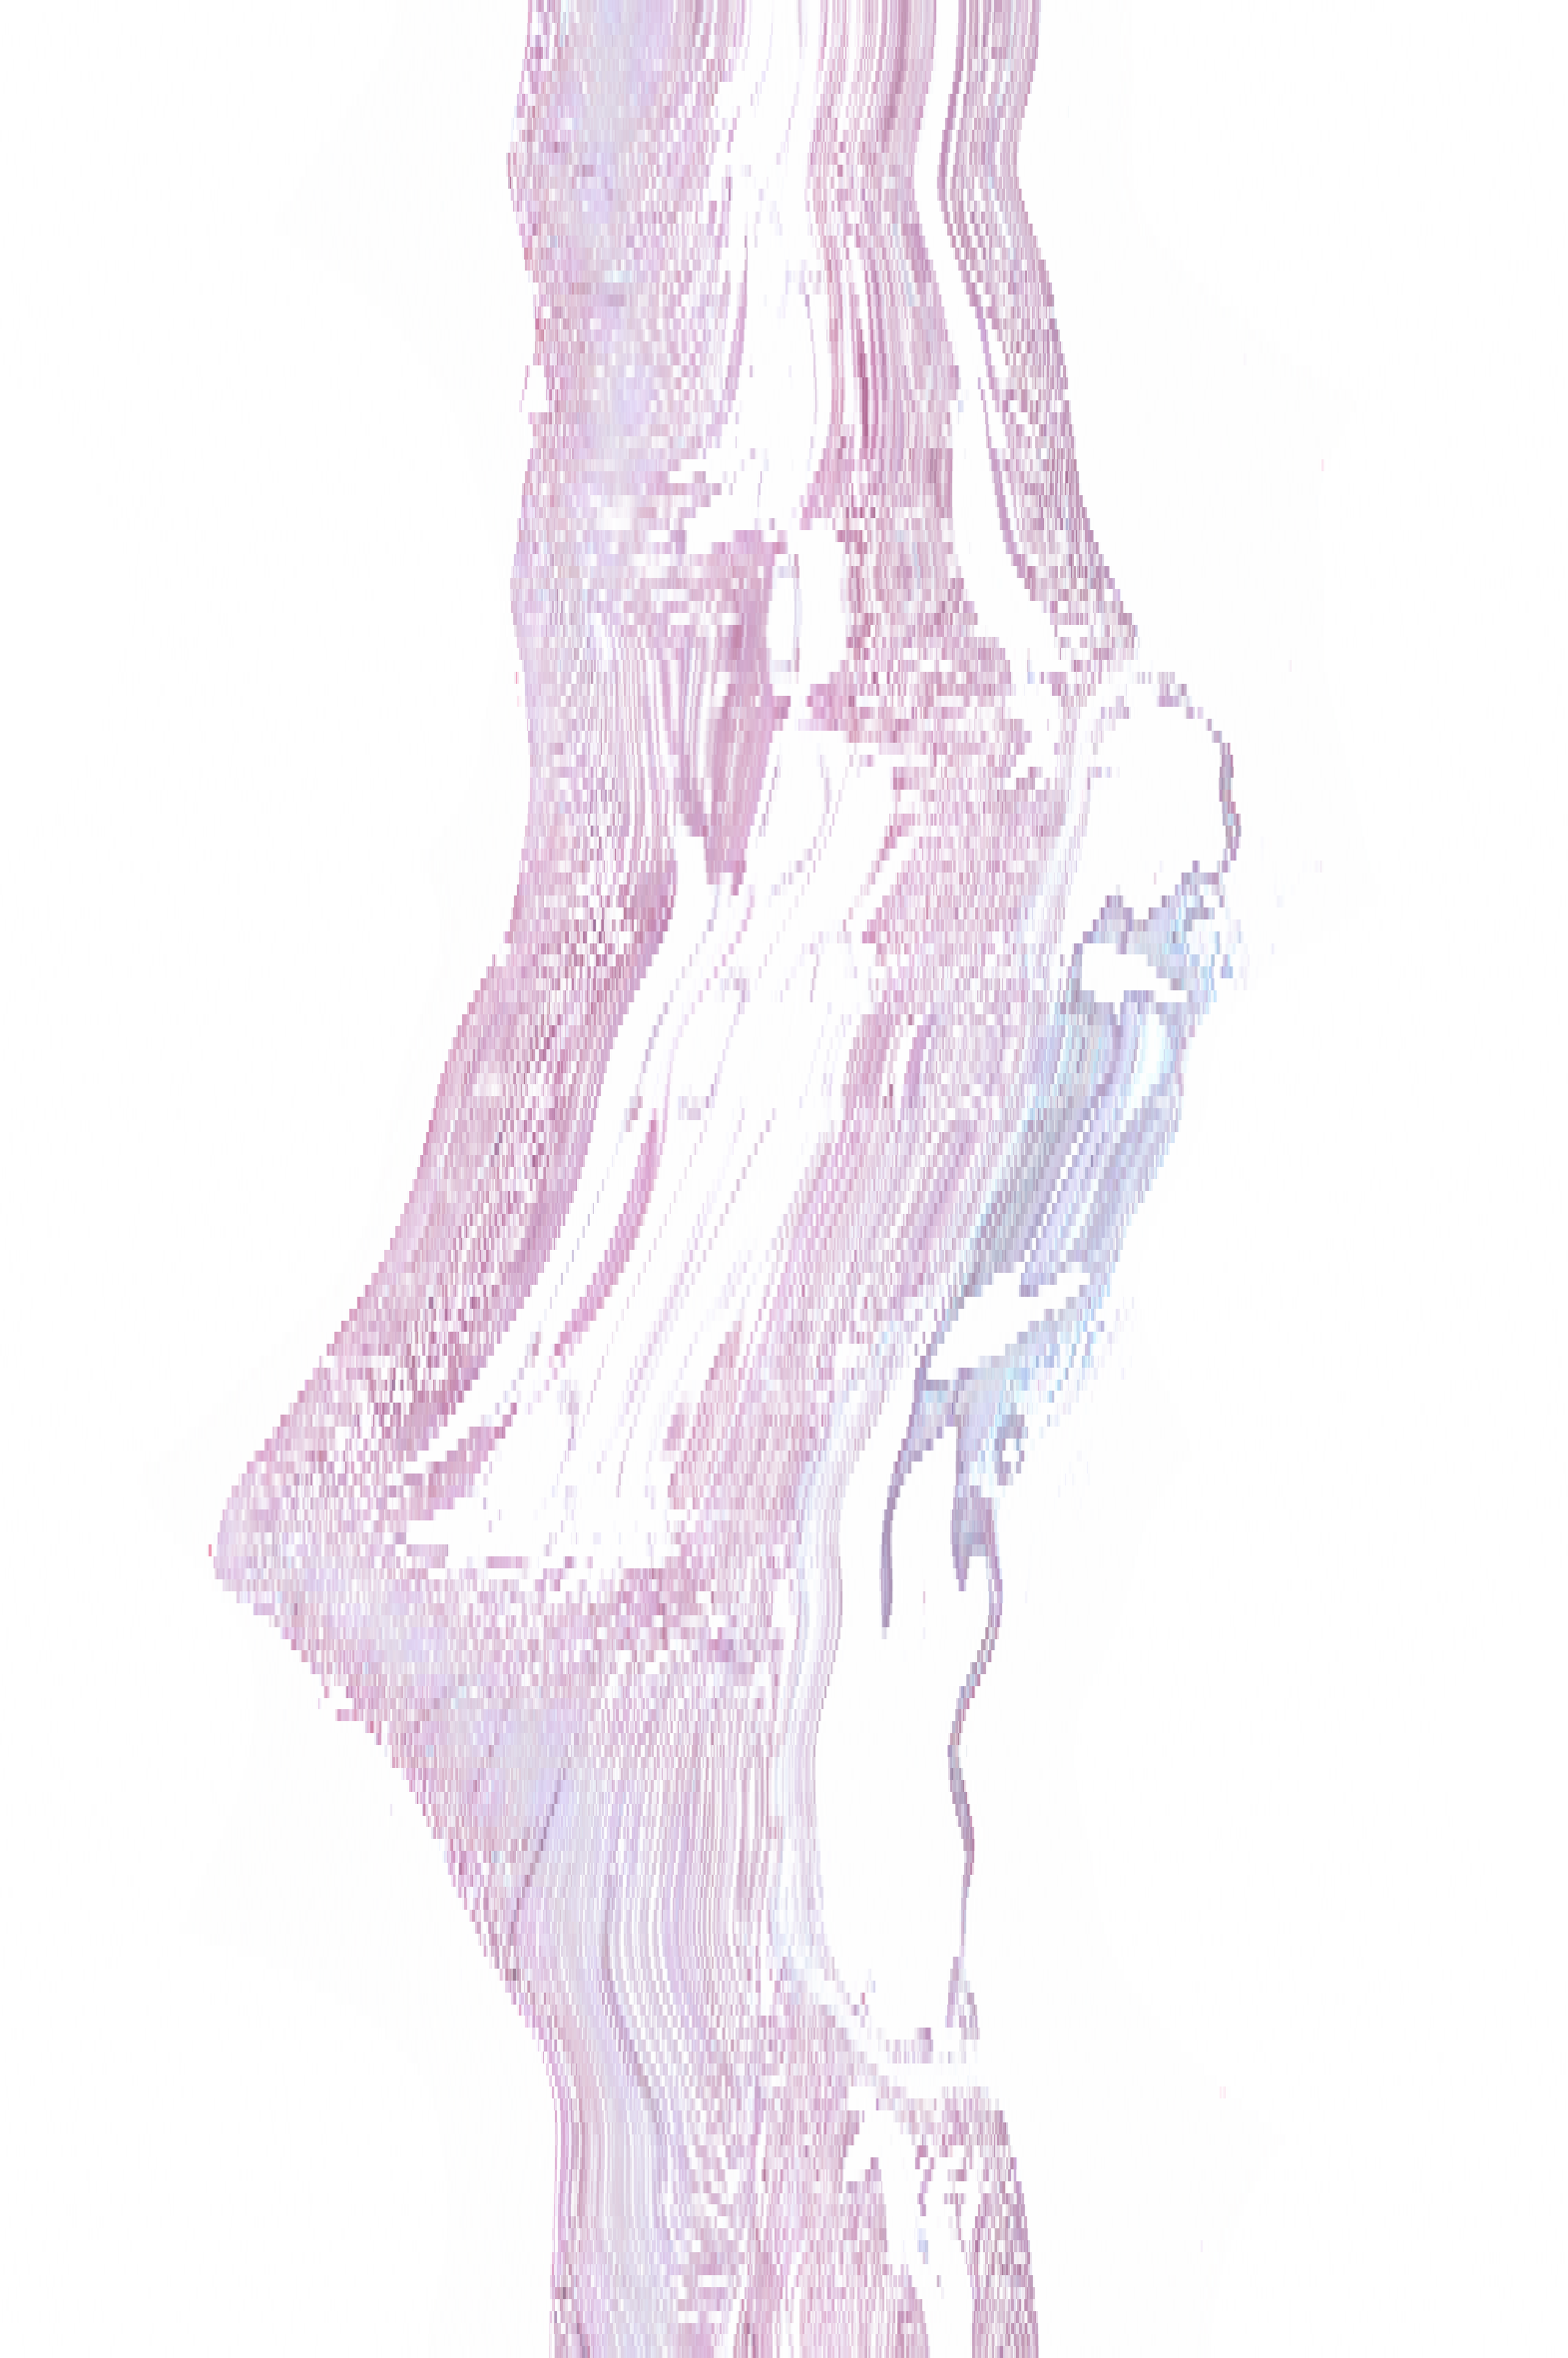
\includegraphics[width=1.1in]{2_methods/Figs/cross_section_40}}
    \subfloat[]{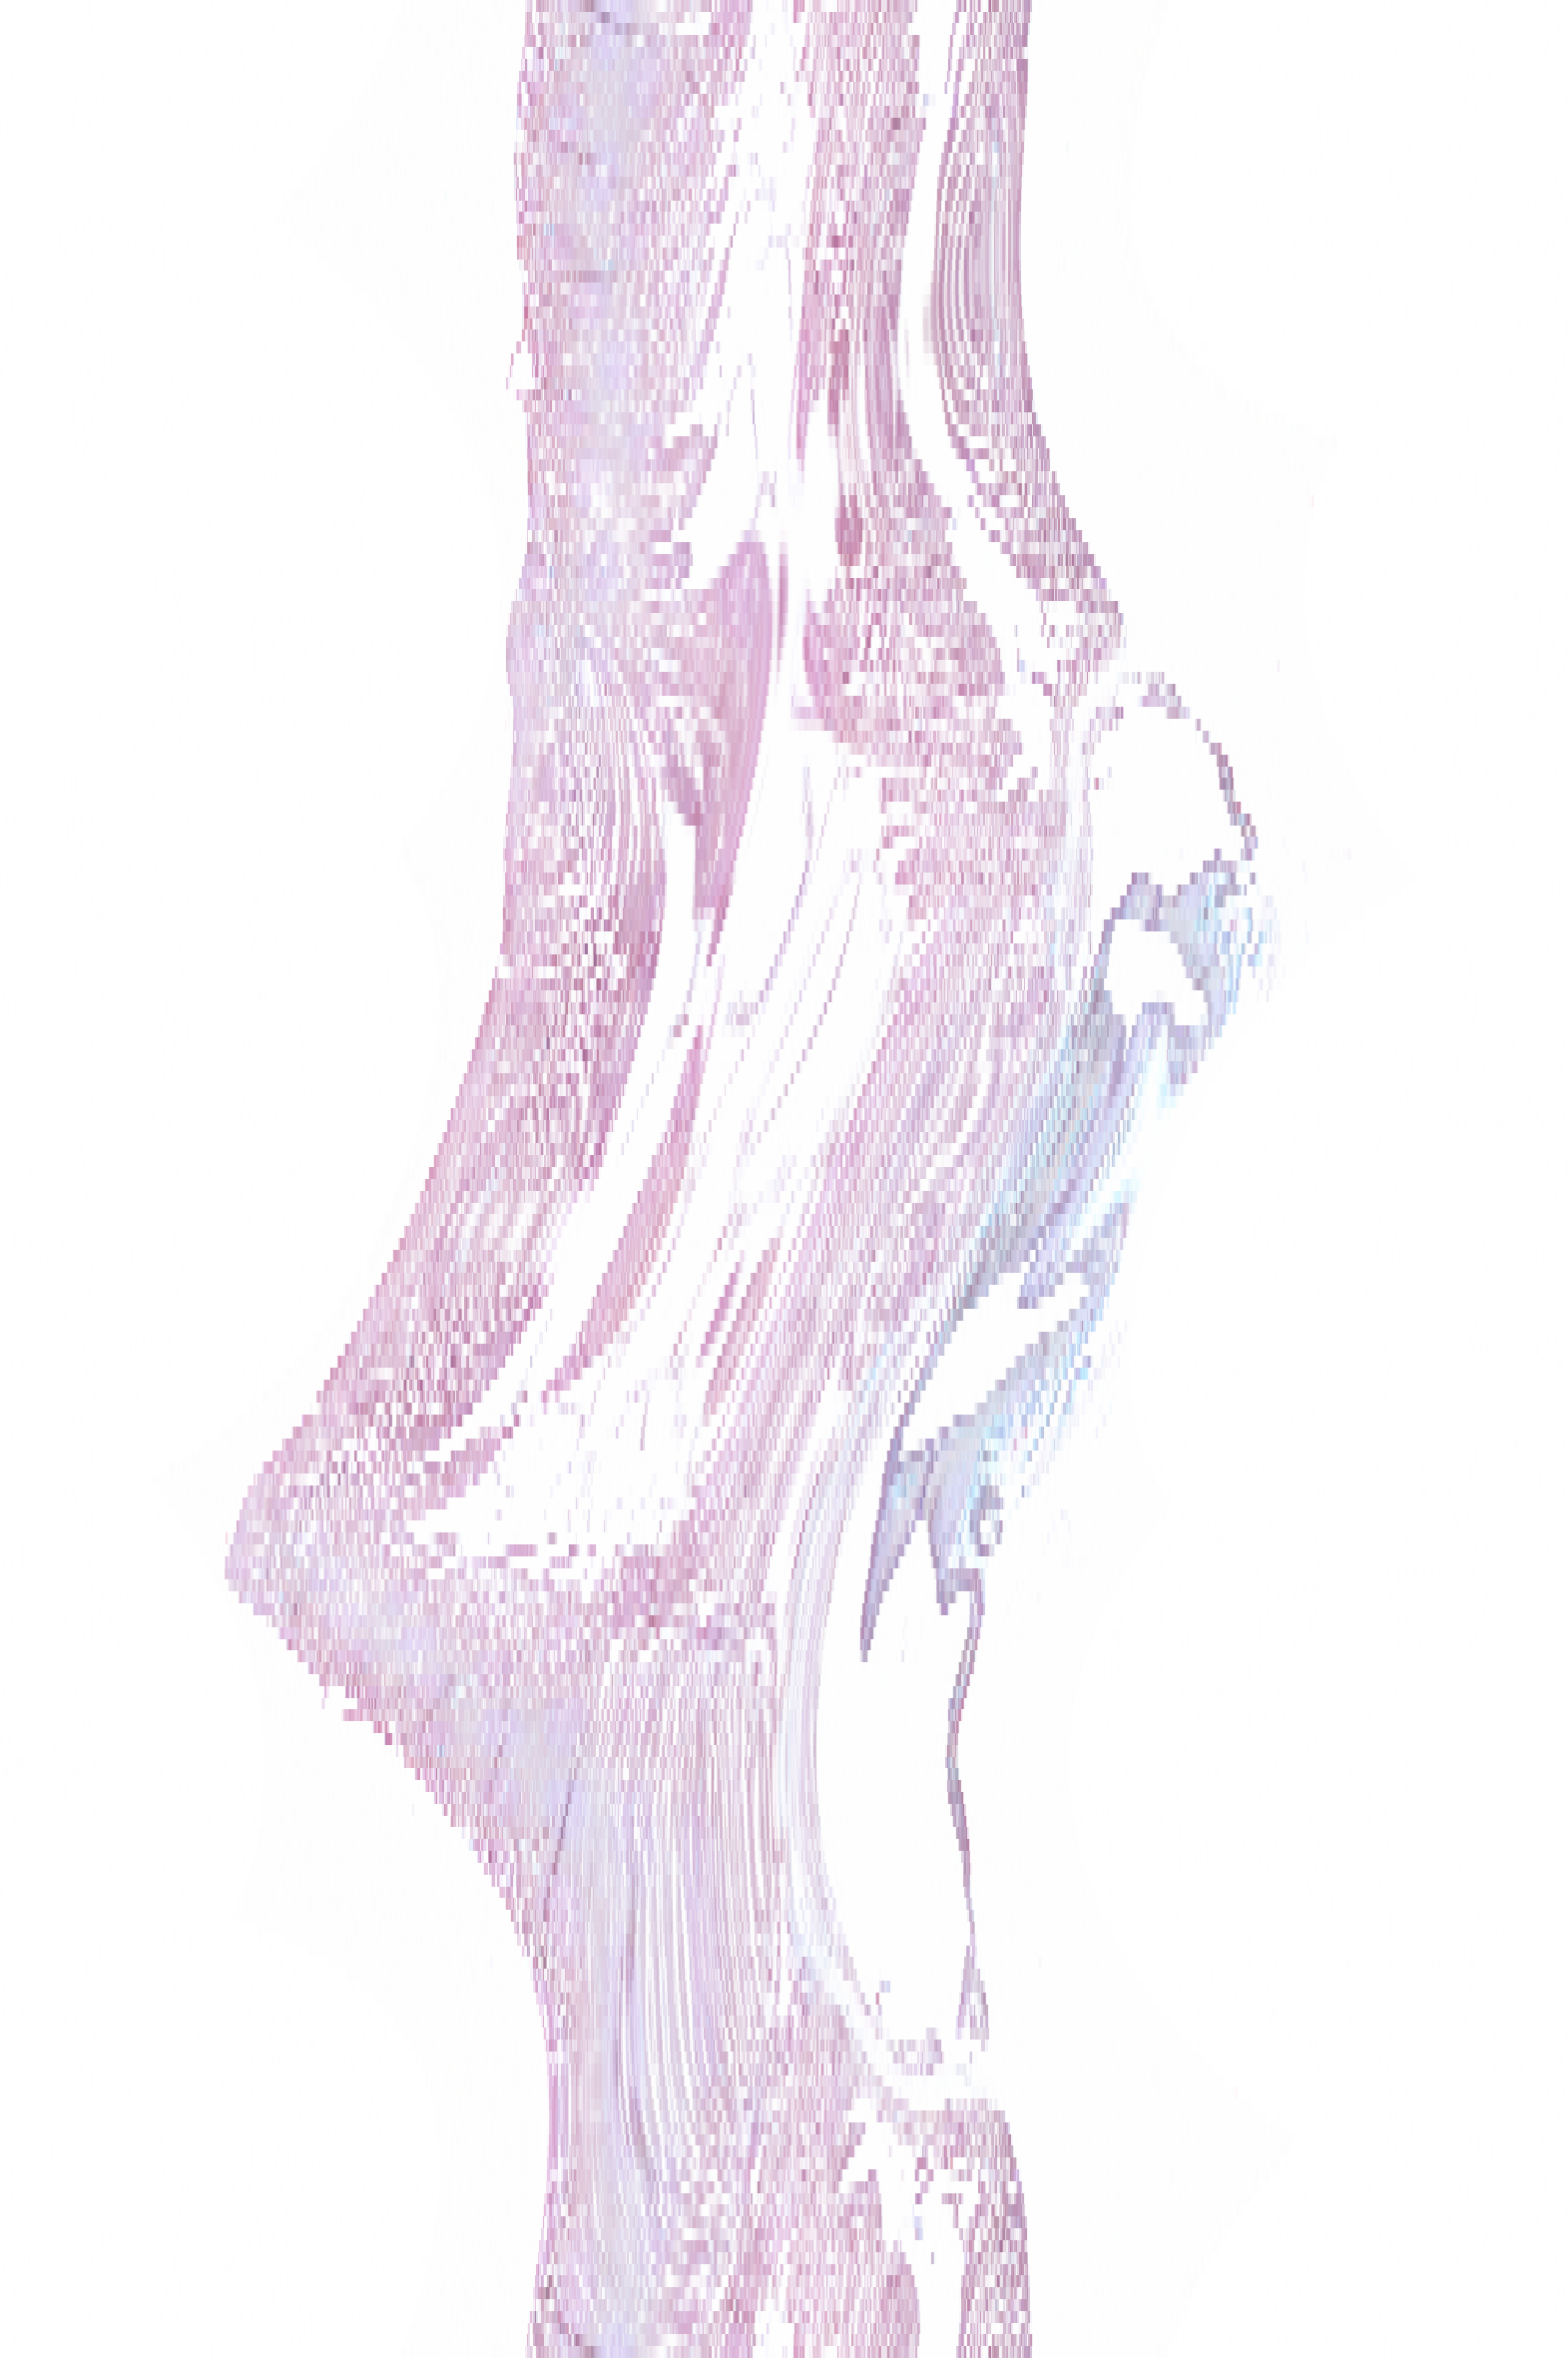
\includegraphics[width=1.1in]{2_methods/Figs/cross_section_perfect}}
    \subfloat[]{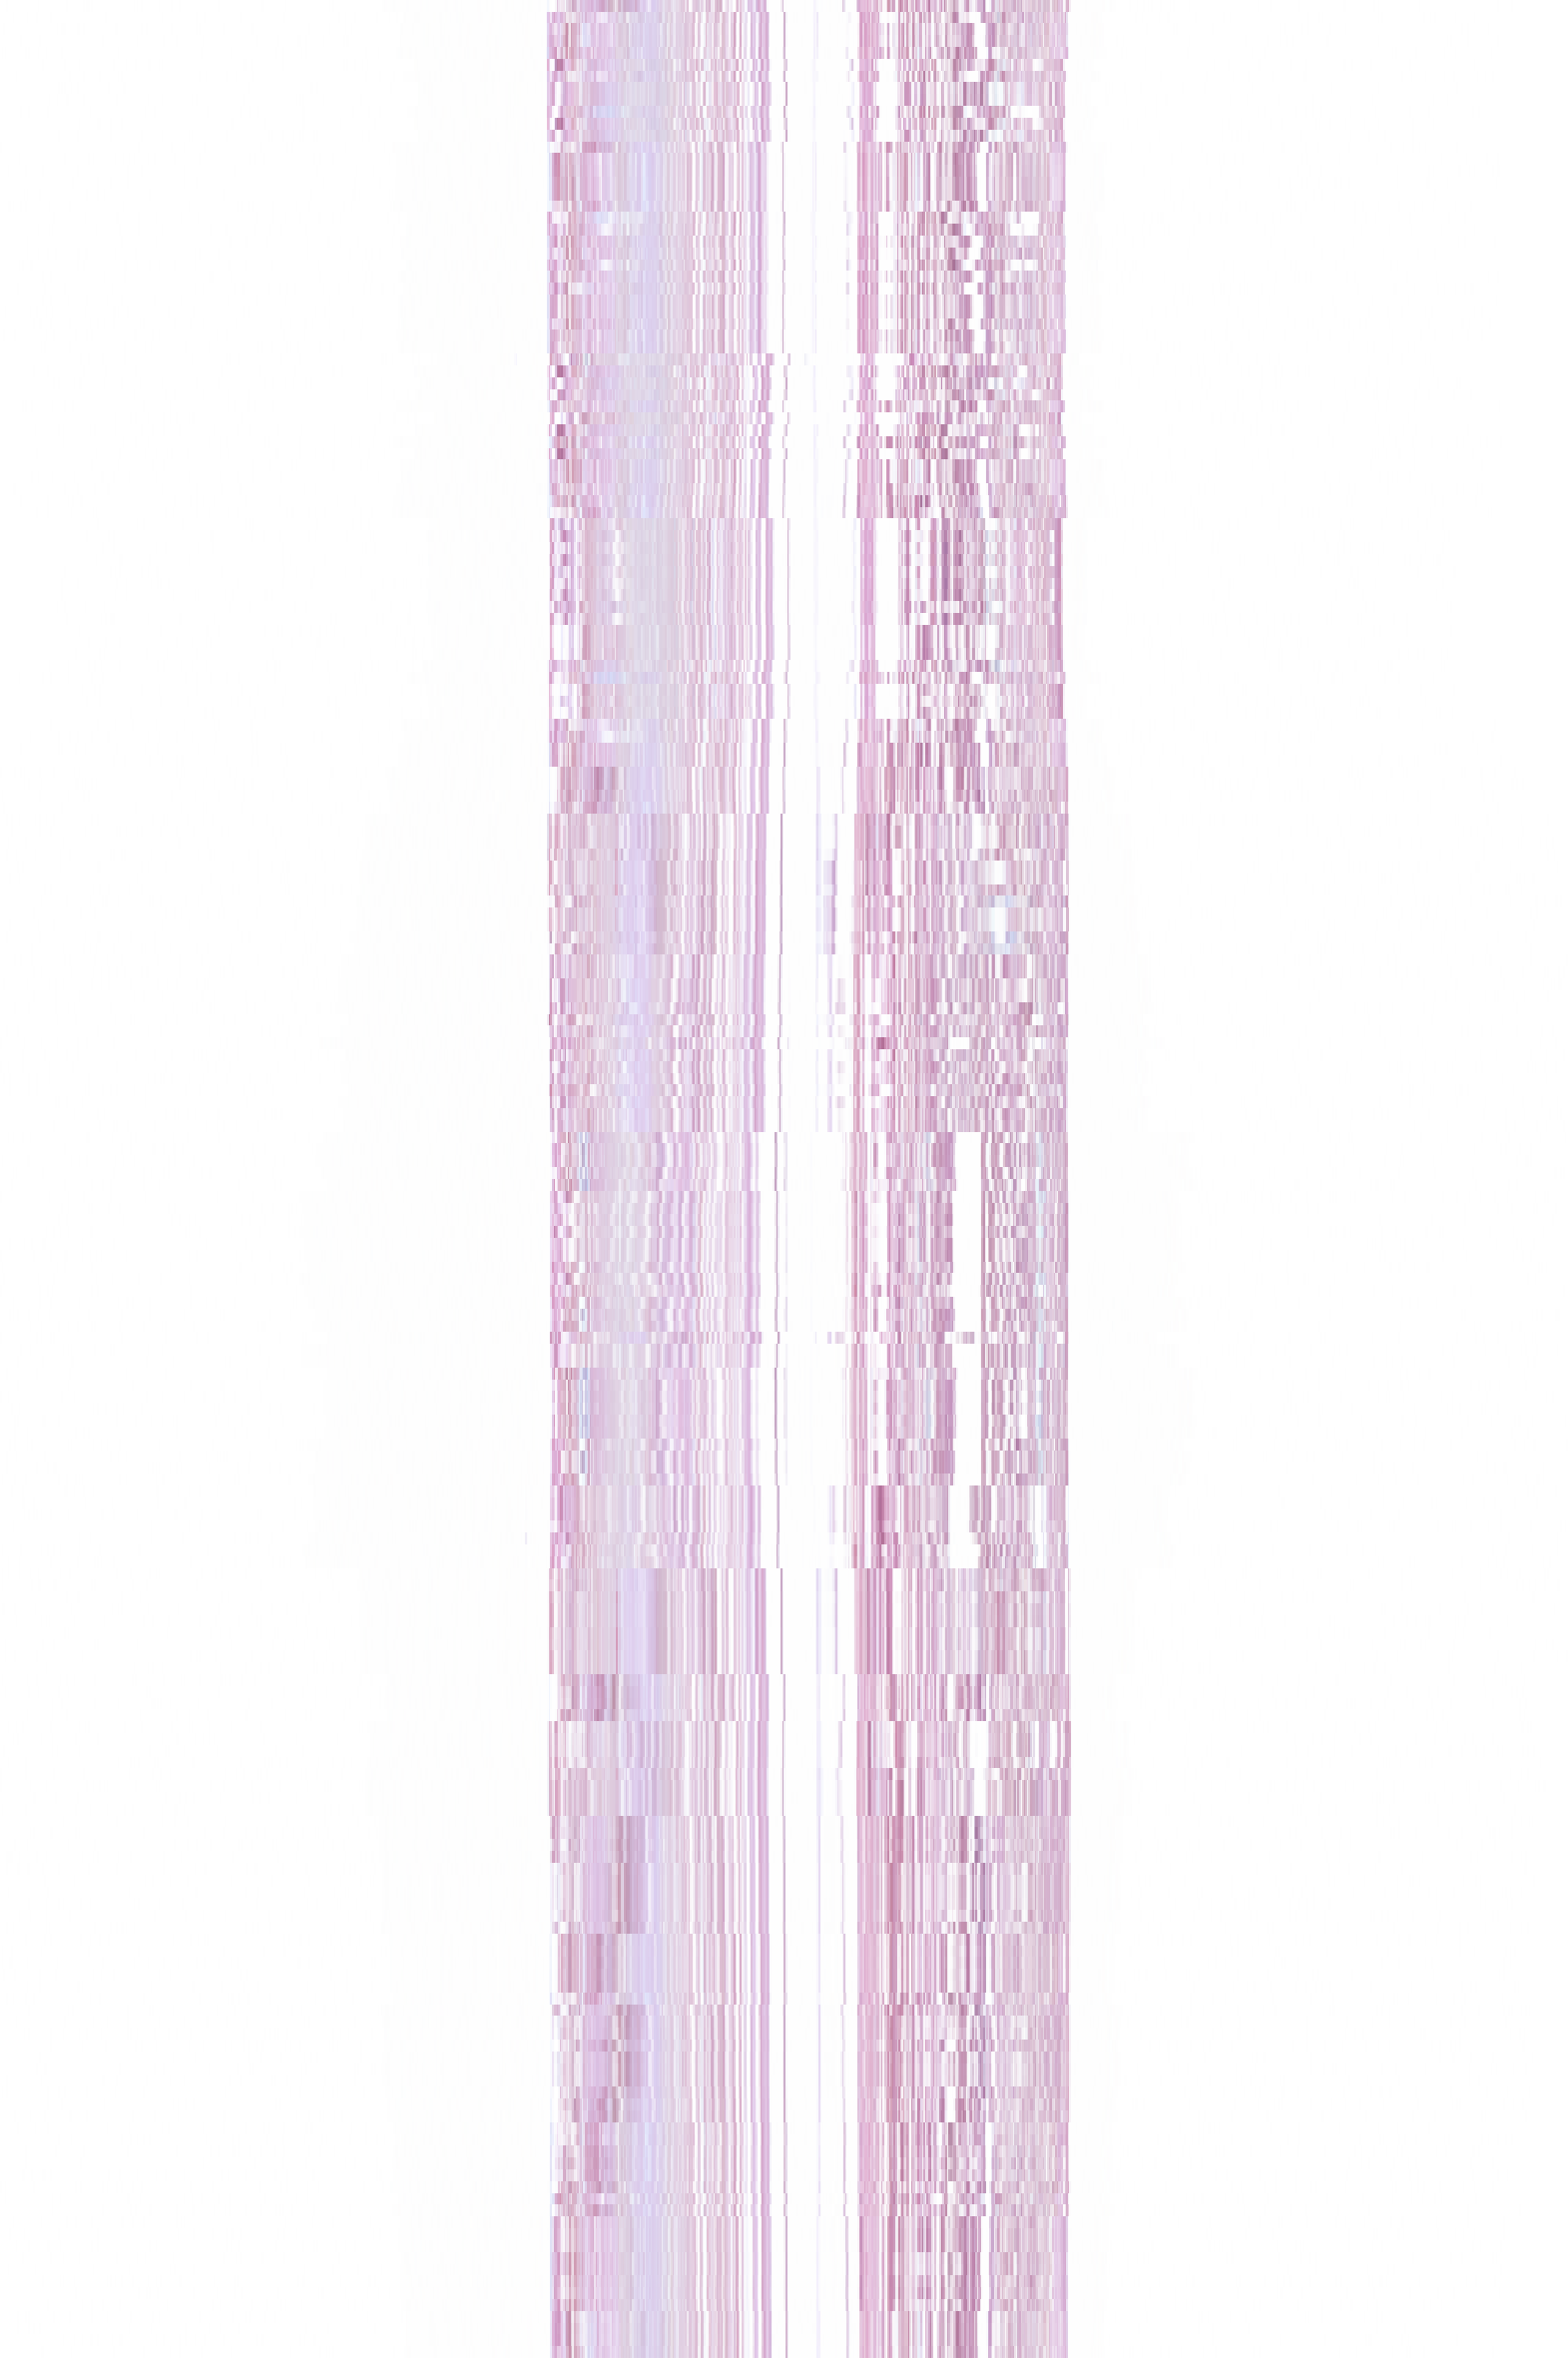
\includegraphics[width=1.1in]{2_methods/Figs/cross_section_banana}}
    \caption{Cross-sections of the synthetic volume (a) before diffusion, (b) after 1 iteration, (c) after 7 iterations and (d) after 40 iterations, with (e) a cross-section of the unperturbed volume as a reference. (f) is the cross-section of a serially registered volume.}
    \label{fig:synthetic_cross_sections}
  \end{figure}
    
  The central cross-sections perpendicular to the x-axes are exhibited in Figure~\ref{fig:synthetic_cross_sections}. Cross-section (a) is of the original unsmoothed noisy volume, and (e) of the volume before noise was added. Three images are sandwiched by these two extremes, of sections smoothed 1, 7 and 40 times. The smoothing performs extremely well on two fronts. By iteration 40, a smooth, continuous section with the appearance of an original histology slice has been recovered from an unrecognisably noisy volume. Secondly and crucially, the underlying geometry of the tissue has been preserved, and the sections appear very similar to the ground truth sections before the noise had been added. Contrastingly, the banana effect is clear from (f), which has lost virtually all of the underlying sinusoidal signal.
  
  \begin{figure}[!t]
    \centering
    \subfloat[]{\includegraphics[width=1.1in]{2_methods/Figs/whole_surface_0}}
    \subfloat[]{\includegraphics[width=1.1in]{2_methods/Figs/whole_surface_1}}
    \subfloat[]{\includegraphics[width=1.1in]{2_methods/Figs/whole_surface_7}}\\
    \subfloat[]{\includegraphics[width=1.1in]{2_methods/Figs/whole_surface_40}}
    \subfloat[]{\includegraphics[width=1.1in]{2_methods/Figs/whole_surface_banana}}
    \caption{Contours of the perturbed synthetic volumes in red before diffusion (a), and after 1 (b), 7 (c) and 40 (d) iterations, overlayed with the unperturbed volume in green. A contour of the serially registered volume in green is shown in (e).}
    \label{fig:synthetic_contours}
  \end{figure}
  
  The nature of the 3-D geometry of the volumes --- the rotation and translation signals, and the transformational noise --- is most clearly understood from the segmentation volume isosurfaces in Figure~\ref{fig:synthetic_contours}. Each of the 4 levels of smoothing depicted by Figure~\ref{fig:synthetic_cross_sections} are overlayed in red with the unperturbed volume in green. Again, the smoothing brings the noisy volume much more closely in line with the ground truth, with the largest effect on the higher frequencies of noise. The conservation of the underlying structure is most evident in Figure~\ref{fig:synthetic_contours}~(d), where the red isosurface deviates almost imperceptibly from the green. The surface of (e) is greatly more discontinous than the red surface of (d), each slice pair having only been coregistered once.

  % Evolution of error from ground truth
  \begin{figure}[!t]
    \subfloat[]{\includegraphics[width=1.7in]{2_methods/Figs/absolute_errors_2d}\label{fig:absolute_errors_2d}}
    \subfloat[]{\includegraphics[width=1.7in]{2_methods/Figs/relative_errors_2d}\label{fig:relative_errors_2d}}
    \caption{Slicewise absolute (a) and relative (b) mean pixel Euclidean distance errors of the initial (blue), final (green) and sequentially registered (red) synthetic volumes. The absolute volumewise means are 1392.696705, 271.5550335 and 4203.940815 and the relative means are 1929.23881407, 37.93561276 and 134.80517588, for the initial, final and sequential volumes respectively.}
    \label{fig:synthetic_errors}
  \end{figure}
  
  Figure~\ref{fig:synthetic_errors}~(a) graphs the mean Euclidean distance of the pixels within a segmentation of the slice from their unperturbed ground truth position, before and after smoothing, and after serial registration. Almost ubiquitously, the metric is greatly reduced after transformational diffusion, evidence that each slice is much more closely aligned to its true position. The overall sinusoidal nature of the serial registration is of course due to the loss of the ground truth morphology. The error after diffusion is prominently the smoothest of the three lines, reflecting the continuity of the volume and the preferential damping of the high frequency spectrum.

  Mean relative Euclidean errors in Figure~\ref{fig:synthetic_errors}~(b) --- distances of pixels in slice $n+1$ from their ground truth positions, both measured from the respective reference frames of slice $n$ --- are cleanly separated on a log scale. The same spectral patterns are observed. Volumewise absolute error is reduced by a factor of 5.1 and relative error by 50 after transformational diffusion smoothing.
% section methods (end)
